\documentclass[]{article}
\usepackage{lmodern}
\usepackage{amssymb,amsmath}
\usepackage{ifxetex,ifluatex}
\usepackage{fixltx2e} % provides \textsubscript
\ifnum 0\ifxetex 1\fi\ifluatex 1\fi=0 % if pdftex
  \usepackage[T1]{fontenc}
  \usepackage[utf8]{inputenc}
\else % if luatex or xelatex
  \ifxetex
    \usepackage{mathspec}
  \else
    \usepackage{fontspec}
  \fi
  \defaultfontfeatures{Ligatures=TeX,Scale=MatchLowercase}
\fi
% use upquote if available, for straight quotes in verbatim environments
\IfFileExists{upquote.sty}{\usepackage{upquote}}{}
% use microtype if available
\IfFileExists{microtype.sty}{%
\usepackage{microtype}
\UseMicrotypeSet[protrusion]{basicmath} % disable protrusion for tt fonts
}{}
\usepackage[margin=1in]{geometry}
\usepackage{hyperref}
\hypersetup{unicode=true,
            pdftitle={Group 7 - Groupwork on leding club loan data},
            pdfauthor={L. Becker, A. Chebatarova, A. Kandel, A.Kusche, R. Mizrak},
            pdfborder={0 0 0},
            breaklinks=true}
\urlstyle{same}  % don't use monospace font for urls
\usepackage{color}
\usepackage{fancyvrb}
\newcommand{\VerbBar}{|}
\newcommand{\VERB}{\Verb[commandchars=\\\{\}]}
\DefineVerbatimEnvironment{Highlighting}{Verbatim}{commandchars=\\\{\}}
% Add ',fontsize=\small' for more characters per line
\usepackage{framed}
\definecolor{shadecolor}{RGB}{248,248,248}
\newenvironment{Shaded}{\begin{snugshade}}{\end{snugshade}}
\newcommand{\AlertTok}[1]{\textcolor[rgb]{0.94,0.16,0.16}{#1}}
\newcommand{\AnnotationTok}[1]{\textcolor[rgb]{0.56,0.35,0.01}{\textbf{\textit{#1}}}}
\newcommand{\AttributeTok}[1]{\textcolor[rgb]{0.77,0.63,0.00}{#1}}
\newcommand{\BaseNTok}[1]{\textcolor[rgb]{0.00,0.00,0.81}{#1}}
\newcommand{\BuiltInTok}[1]{#1}
\newcommand{\CharTok}[1]{\textcolor[rgb]{0.31,0.60,0.02}{#1}}
\newcommand{\CommentTok}[1]{\textcolor[rgb]{0.56,0.35,0.01}{\textit{#1}}}
\newcommand{\CommentVarTok}[1]{\textcolor[rgb]{0.56,0.35,0.01}{\textbf{\textit{#1}}}}
\newcommand{\ConstantTok}[1]{\textcolor[rgb]{0.00,0.00,0.00}{#1}}
\newcommand{\ControlFlowTok}[1]{\textcolor[rgb]{0.13,0.29,0.53}{\textbf{#1}}}
\newcommand{\DataTypeTok}[1]{\textcolor[rgb]{0.13,0.29,0.53}{#1}}
\newcommand{\DecValTok}[1]{\textcolor[rgb]{0.00,0.00,0.81}{#1}}
\newcommand{\DocumentationTok}[1]{\textcolor[rgb]{0.56,0.35,0.01}{\textbf{\textit{#1}}}}
\newcommand{\ErrorTok}[1]{\textcolor[rgb]{0.64,0.00,0.00}{\textbf{#1}}}
\newcommand{\ExtensionTok}[1]{#1}
\newcommand{\FloatTok}[1]{\textcolor[rgb]{0.00,0.00,0.81}{#1}}
\newcommand{\FunctionTok}[1]{\textcolor[rgb]{0.00,0.00,0.00}{#1}}
\newcommand{\ImportTok}[1]{#1}
\newcommand{\InformationTok}[1]{\textcolor[rgb]{0.56,0.35,0.01}{\textbf{\textit{#1}}}}
\newcommand{\KeywordTok}[1]{\textcolor[rgb]{0.13,0.29,0.53}{\textbf{#1}}}
\newcommand{\NormalTok}[1]{#1}
\newcommand{\OperatorTok}[1]{\textcolor[rgb]{0.81,0.36,0.00}{\textbf{#1}}}
\newcommand{\OtherTok}[1]{\textcolor[rgb]{0.56,0.35,0.01}{#1}}
\newcommand{\PreprocessorTok}[1]{\textcolor[rgb]{0.56,0.35,0.01}{\textit{#1}}}
\newcommand{\RegionMarkerTok}[1]{#1}
\newcommand{\SpecialCharTok}[1]{\textcolor[rgb]{0.00,0.00,0.00}{#1}}
\newcommand{\SpecialStringTok}[1]{\textcolor[rgb]{0.31,0.60,0.02}{#1}}
\newcommand{\StringTok}[1]{\textcolor[rgb]{0.31,0.60,0.02}{#1}}
\newcommand{\VariableTok}[1]{\textcolor[rgb]{0.00,0.00,0.00}{#1}}
\newcommand{\VerbatimStringTok}[1]{\textcolor[rgb]{0.31,0.60,0.02}{#1}}
\newcommand{\WarningTok}[1]{\textcolor[rgb]{0.56,0.35,0.01}{\textbf{\textit{#1}}}}
\usepackage{graphicx,grffile}
\makeatletter
\def\maxwidth{\ifdim\Gin@nat@width>\linewidth\linewidth\else\Gin@nat@width\fi}
\def\maxheight{\ifdim\Gin@nat@height>\textheight\textheight\else\Gin@nat@height\fi}
\makeatother
% Scale images if necessary, so that they will not overflow the page
% margins by default, and it is still possible to overwrite the defaults
% using explicit options in \includegraphics[width, height, ...]{}
\setkeys{Gin}{width=\maxwidth,height=\maxheight,keepaspectratio}
\IfFileExists{parskip.sty}{%
\usepackage{parskip}
}{% else
\setlength{\parindent}{0pt}
\setlength{\parskip}{6pt plus 2pt minus 1pt}
}
\setlength{\emergencystretch}{3em}  % prevent overfull lines
\providecommand{\tightlist}{%
  \setlength{\itemsep}{0pt}\setlength{\parskip}{0pt}}
\setcounter{secnumdepth}{0}
% Redefines (sub)paragraphs to behave more like sections
\ifx\paragraph\undefined\else
\let\oldparagraph\paragraph
\renewcommand{\paragraph}[1]{\oldparagraph{#1}\mbox{}}
\fi
\ifx\subparagraph\undefined\else
\let\oldsubparagraph\subparagraph
\renewcommand{\subparagraph}[1]{\oldsubparagraph{#1}\mbox{}}
\fi

%%% Use protect on footnotes to avoid problems with footnotes in titles
\let\rmarkdownfootnote\footnote%
\def\footnote{\protect\rmarkdownfootnote}

%%% Change title format to be more compact
\usepackage{titling}

% Create subtitle command for use in maketitle
\providecommand{\subtitle}[1]{
  \posttitle{
    \begin{center}\large#1\end{center}
    }
}

\setlength{\droptitle}{-2em}

  \title{Group 7 - Groupwork on leding club loan data}
    \pretitle{\vspace{\droptitle}\centering\huge}
  \posttitle{\par}
    \author{L. Becker, A. Chebatarova, A. Kandel, A.Kusche, R. Mizrak}
    \preauthor{\centering\large\emph}
  \postauthor{\par}
      \predate{\centering\large\emph}
  \postdate{\par}
    \date{2019-05-26}


\begin{document}
\maketitle

\hypertarget{introduction}{%
\section{Introduction}\label{introduction}}

Our data comes from Lending Club (LC) which is a peer-to-peer online
lending platform. The data contains information on the loans issued by
LC including the details of the loans such as loan description, interest
rate applied, if the debt was fully paid, date of last payment etc. Our
goal is to find appropriate models for predicting interest rate for each
request, as well as perform classification model for setting reliable
default status.

URL to source data:
\url{https://kaggle.com/wendykan/lending-club-loan-data}

Required steps:

\begin{itemize}
\item
  Initialization of the environment.
\item
  Data exploration through data visualization which helps to understand
  our dataset and its characteristics.
\item
  Data preprocessing which includes omitting unnecessary columns,
  sorting and grouping, reformatting and other actions required for
  making our data adequate for performing further analysis and modeling.
\item
  Part 1: Regression Analysis - we get into details with our data to
  define meaningful amount of data, rational predictors, check
  correlations and determine models for prediction of interest rate and
  validate them.
\item
  Part 2 - Classification Analysis - we take a step back in order to be
  sure that all necessary variables are included into our analysis,
  perform required transformations, define the models, check the errors
  and validate the results.
\item
  Summary
\end{itemize}

\hypertarget{initializing-the-environment}{%
\section{Initializing the
environment}\label{initializing-the-environment}}

At this step we clear the workspace and install necessary packages for
data processing.

\begin{Shaded}
\begin{Highlighting}[]
  \CommentTok{# Clear objects from the workspace}
  \KeywordTok{rm}\NormalTok{(}\DataTypeTok{list=}\NormalTok{(}\KeywordTok{ls}\NormalTok{()))}
  
  \CommentTok{# load library to deal with packages}
  \KeywordTok{library}\NormalTok{(pacman)}

  \CommentTok{# install and loading required packages}
\NormalTok{  pacman}\OperatorTok{::}\KeywordTok{p_load}\NormalTok{(import, monomvn, party, dummies, ranger, data.table, rmarkdown, tidyverse, }
\NormalTok{  caret, pls, corrplot, randomForest, foreach, plyr, tidyverse, magrittr, dplyr, tibble, doMC, }
\NormalTok{  pROC, class,MLmetrics, tree, car, ridge, lmridge, xgboost)}
\end{Highlighting}
\end{Shaded}

\begin{verbatim}
## Installing package into 'C:/Users/Startklar/Documents/R/win-library/3.6'
## (as 'lib' is unspecified)
\end{verbatim}

\begin{verbatim}
## Warning: package 'doMC' is not available (for R version 3.6.0)
\end{verbatim}

\begin{verbatim}
## Warning: unable to access index for repository http://www.stats.ox.ac.uk/pub/RWin/bin/windows/contrib/3.6:
##   cannot open URL 'http://www.stats.ox.ac.uk/pub/RWin/bin/windows/contrib/3.6/PACKAGES'
\end{verbatim}

\begin{verbatim}
## Warning: 'BiocManager' not available.  Could not check Bioconductor.
## 
## Please use `install.packages('BiocManager')` and then retry.
\end{verbatim}

\begin{verbatim}
## Warning in p_install(package, character.only = TRUE, ...):
\end{verbatim}

\begin{verbatim}
## Warning in library(package, lib.loc = lib.loc, character.only = TRUE,
## logical.return = TRUE, : there is no package called 'doMC'
\end{verbatim}

\begin{verbatim}
## Warning in pacman::p_load(import, monomvn, party, dummies, ranger, data.table, : Failed to install/load:
## doMC
\end{verbatim}

\pagebreak

\hypertarget{data-extraction}{%
\section{Data Extraction}\label{data-extraction}}

In order to avoid to have to work with the whole original dataset from
kaggle dataset\_7.Rds has been created as follows:

Read the subset of data from the previous step

\begin{Shaded}
\begin{Highlighting}[]
\CommentTok{# Read the RDS file}
\NormalTok{dataset <-}\StringTok{ }\KeywordTok{readRDS}\NormalTok{(}\DataTypeTok{file =} \StringTok{"dataset_7.Rds"}\NormalTok{)}
\CommentTok{# Setting seed}
\KeywordTok{set.seed}\NormalTok{(}\DecValTok{3452}\NormalTok{)}
\NormalTok{dataset <-}\StringTok{ }\NormalTok{dataset[}\KeywordTok{sample}\NormalTok{(}\DecValTok{1}\OperatorTok{:}\KeywordTok{nrow}\NormalTok{(dataset),}\DecValTok{20000}\NormalTok{),]}
\end{Highlighting}
\end{Shaded}

\hypertarget{data-preprocessing}{%
\section{Data Preprocessing}\label{data-preprocessing}}

Preprocess the dataset, remove colums, check for na \ldots{}

\begin{Shaded}
\begin{Highlighting}[]
  \CommentTok{# sort dataset by colunm names, to facilite search}
\NormalTok{  dataset =}\StringTok{ }\NormalTok{dataset[ , }\KeywordTok{order}\NormalTok{(}\KeywordTok{names}\NormalTok{(dataset))]}
  
  \CommentTok{# Removing columns that have > 0.05 NAs}
\NormalTok{  dataset <-}\StringTok{ }\NormalTok{dataset[, }\OperatorTok{-}\KeywordTok{which}\NormalTok{(}\KeywordTok{colMeans}\NormalTok{(}\KeywordTok{is.na}\NormalTok{(dataset)) }\OperatorTok{>}\StringTok{ }\FloatTok{0.05}\NormalTok{)]}
  
  \CommentTok{# remove some columsn because of the reasons below }
  \CommentTok{# to many levels: zip_code, emp_title}
  \CommentTok{# not_relevant: desc, id_2, addr_state, last_pymnt_d, next_pymnt_d, issue_d, title, last_credit_pull_d, hardship_end_date, hardship_start_date, payment_plan_start_date, debt_settlement_flag_date, settlement_date}
  \CommentTok{# same data in every colum: policy_code}
  \CommentTok{# covariance: grade (of sub_grade)}
  
\NormalTok{  dataset <-}\StringTok{ }\KeywordTok{subset}\NormalTok{(dataset, }\DataTypeTok{select =} \OperatorTok{-}\KeywordTok{c}\NormalTok{(id_}\DecValTok{2}\NormalTok{, policy_code, desc, emp_title, issue_d, title, zip_code, last_pymnt_d, next_pymnt_d, last_credit_pull_d, hardship_end_date, hardship_start_date, payment_plan_start_date, debt_settlement_flag_date, settlement_date, addr_state, grade) )}

  \CommentTok{# sub_grade has more than 32 levels which is a hard limit for random forest.}
  \CommentTok{# We'll dummy code it to circument this}
\NormalTok{  levels_sub_grade <-}\StringTok{ }\KeywordTok{levels}\NormalTok{(dataset}\OperatorTok{$}\NormalTok{sub_grade)}
\NormalTok{  dataset}\OperatorTok{$}\NormalTok{sub_grade<-}\StringTok{ }\KeywordTok{as.numeric}\NormalTok{(}\KeywordTok{mapvalues}\NormalTok{(dataset}\OperatorTok{$}\NormalTok{sub_grade, levels_sub_grade, }\KeywordTok{seq}\NormalTok{(}\DataTypeTok{from =} \DecValTok{1}\NormalTok{, }\DataTypeTok{to =} \DecValTok{35}\NormalTok{, }\DataTypeTok{by =} \DecValTok{1}\NormalTok{)))}

  
  \CommentTok{# sorting emp_lenght, and dummy coding.}
\NormalTok{  levels_emp_length <-}\StringTok{ }\KeywordTok{levels}\NormalTok{(dataset}\OperatorTok{$}\NormalTok{emp_length)}
\NormalTok{  dataset}\OperatorTok{$}\NormalTok{emp_length <-}\StringTok{ }\KeywordTok{ordered}\NormalTok{(dataset}\OperatorTok{$}\NormalTok{emp_length, }\DataTypeTok{levels =} \KeywordTok{c}\NormalTok{(}\StringTok{"n/a"}\NormalTok{, }\StringTok{"< 1 year"}\NormalTok{, }\StringTok{"1 year"}\NormalTok{, }\StringTok{"2 years"}\NormalTok{, }\StringTok{"3 years"}\NormalTok{,}\StringTok{"4 years"}\NormalTok{, }\StringTok{"5 years"}\NormalTok{,}\StringTok{"6 years"}\NormalTok{, }\StringTok{"7 years"}\NormalTok{, }\StringTok{"8 years"}\NormalTok{, }\StringTok{"9 years"}\NormalTok{, }\StringTok{"10+ years"}\NormalTok{))}
  \KeywordTok{levels}\NormalTok{(dataset}\OperatorTok{$}\NormalTok{emp_length)}
\end{Highlighting}
\end{Shaded}

\begin{verbatim}
##  [1] "n/a"       "< 1 year"  "1 year"    "2 years"   "3 years"  
##  [6] "4 years"   "5 years"   "6 years"   "7 years"   "8 years"  
## [11] "9 years"   "10+ years"
\end{verbatim}

\begin{Shaded}
\begin{Highlighting}[]
\NormalTok{  dataset}\OperatorTok{$}\NormalTok{emp_length <-}\StringTok{ }\KeywordTok{as.numeric}\NormalTok{(}\KeywordTok{mapvalues}\NormalTok{(dataset}\OperatorTok{$}\NormalTok{emp_length, levels_emp_length, }\KeywordTok{c}\NormalTok{(}\OperatorTok{-}\DecValTok{1}\NormalTok{, }\KeywordTok{seq}\NormalTok{(}\DataTypeTok{from =} \DecValTok{0}\NormalTok{, }\DataTypeTok{to =} \DecValTok{10}\NormalTok{, }\DataTypeTok{by =} \DecValTok{1}\NormalTok{))))}

  
  \CommentTok{# grouping earliest_cr_line by year}
\NormalTok{  dataset}\OperatorTok{$}\NormalTok{earliest_cr_line <-}\StringTok{ }\KeywordTok{as.integer}\NormalTok{(}\KeywordTok{substring}\NormalTok{(dataset}\OperatorTok{$}\NormalTok{earliest_cr_line, }\DecValTok{5}\NormalTok{))}
  
  \CommentTok{# grouping earliest_cr_line by year}
\NormalTok{  dataset}\OperatorTok{$}\NormalTok{sec_app_earliest_cr_line <-}\StringTok{ }\KeywordTok{as.integer}\NormalTok{(}\KeywordTok{substring}\NormalTok{(}\KeywordTok{as.character}\NormalTok{(dataset}\OperatorTok{$}\NormalTok{sec_app_earliest_cr_line), }\DecValTok{5}\NormalTok{))}
\NormalTok{  dataset}\OperatorTok{$}\NormalTok{sec_app_earliest_cr_line[}\KeywordTok{is.na}\NormalTok{(dataset}\OperatorTok{$}\NormalTok{sec_app_earliest_cr_line)] <-}\StringTok{ }\DecValTok{-1}
  \KeywordTok{typeof}\NormalTok{(dataset}\OperatorTok{$}\NormalTok{sec_app_earliest_cr_line)}
\end{Highlighting}
\end{Shaded}

\begin{verbatim}
## [1] "double"
\end{verbatim}

\begin{Shaded}
\begin{Highlighting}[]
\NormalTok{  na_count <-}\KeywordTok{sapply}\NormalTok{(dataset, }\ControlFlowTok{function}\NormalTok{(y) }\KeywordTok{sum}\NormalTok{(}\KeywordTok{length}\NormalTok{(}\KeywordTok{which}\NormalTok{(}\KeywordTok{is.na}\NormalTok{(y)))))}
  
  \CommentTok{# changing the dataset as a tbl object.}
\NormalTok{  dataset <-}\StringTok{ }\KeywordTok{as.tbl}\NormalTok{(dataset)}
  \CommentTok{# change NAs to 0 in integer columns}
\NormalTok{  dataset <-}\StringTok{ }\KeywordTok{mutate_if}\NormalTok{(dataset, is.integer, }\OperatorTok{~}\KeywordTok{replace}\NormalTok{(., }\KeywordTok{is.na}\NormalTok{(.), }\DecValTok{-1}\NormalTok{))}
  \CommentTok{# change NAs to 0 in doubles columns}
  
\NormalTok{  dataset <-}\StringTok{ }\KeywordTok{mutate_if}\NormalTok{(dataset, is.numeric, }\OperatorTok{~}\KeywordTok{replace}\NormalTok{(., }\KeywordTok{is.na}\NormalTok{(.), }\DecValTok{-1}\NormalTok{))}
  \CommentTok{# change NAs to 0 in strings columns}
  
\NormalTok{  dataset <-}\StringTok{ }\KeywordTok{mutate_if}\NormalTok{(dataset, is.character, }\OperatorTok{~}\KeywordTok{replace}\NormalTok{(., }\KeywordTok{is.na}\NormalTok{(.), }\StringTok{"NA"}\NormalTok{))}
  
  \CommentTok{# change NAs to 0 in strings columns}
  
\NormalTok{  dataset <-}\StringTok{ }\KeywordTok{mutate_if}\NormalTok{(dataset, is.factor, }\OperatorTok{~}\KeywordTok{replace}\NormalTok{(., }\KeywordTok{is.na}\NormalTok{(.), }\StringTok{"NA"}\NormalTok{))}
  
   \CommentTok{# }
\NormalTok{  dataset <-}\StringTok{ }\KeywordTok{mutate_if}\NormalTok{(dataset, is.character, }\OperatorTok{~}\KeywordTok{replace}\NormalTok{(., }\KeywordTok{is.na}\NormalTok{(.), }\StringTok{"NA"}\NormalTok{))}
  \CommentTok{# }
  
  \CommentTok{# calculating the number of unique levels per column}
  \KeywordTok{sapply}\NormalTok{(dataset, }\ControlFlowTok{function}\NormalTok{(col) }\KeywordTok{length}\NormalTok{(}\KeywordTok{unique}\NormalTok{(col)))}
\end{Highlighting}
\end{Shaded}

\begin{verbatim}
##             acc_now_delinq       acc_open_past_24mths 
##                          5                         34 
##                 annual_inc           application_type 
##                       2482                          2 
##                avg_cur_bal             bc_open_to_buy 
##                      13493                      12312 
##                    bc_util   chargeoff_within_12_mths 
##                       1075                          4 
##    collection_recovery_fee collections_12_mths_ex_med 
##                       1500                          5 
##       debt_settlement_flag                delinq_2yrs 
##                          2                         18 
##                delinq_amnt        disbursement_method 
##                         62                          2 
##                        dti           earliest_cr_line 
##                       3862                         56 
##                 emp_length                funded_amnt 
##                         12                       1079 
##            funded_amnt_inv              hardship_flag 
##                       1207                          2 
##       hardship_loan_status            hardship_reason 
##                          5                          9 
##            hardship_status              hardship_type 
##                          4                          2 
##             home_ownership        initial_list_status 
##                          6                          2 
##             inq_last_6mths                installment 
##                         12                      10601 
##                   int_rate            last_pymnt_amnt 
##                        475                      15422 
##                  loan_amnt                loan_status 
##                       1079                          8 
##       mo_sin_old_rev_tl_op      mo_sin_rcnt_rev_tl_op 
##                        571                        155 
##             mo_sin_rcnt_tl                   mort_acc 
##                        102                         18 
##       mths_since_recent_bc      num_accts_ever_120_pd 
##                        239                         20 
##             num_actv_bc_tl            num_actv_rev_tl 
##                         26                         37 
##                num_bc_sats                  num_bc_tl 
##                         33                         43 
##                  num_il_tl              num_op_rev_tl 
##                         69                         44 
##              num_rev_accts        num_rev_tl_bal_gt_0 
##                         64                         33 
##                   num_sats               num_tl_30dpd 
##                         51                          5 
##         num_tl_90g_dpd_24m         num_tl_op_past_12m 
##                         14                         20 
##                   open_acc                  out_prncp 
##                         54                       7727 
##              out_prncp_inv             pct_tl_nvr_dlq 
##                       7763                        347 
##           percent_bc_gt_75                    pub_rec 
##                        110                         11 
##       pub_rec_bankruptcies                    purpose 
##                          7                         14 
##                 pymnt_plan                 recoveries 
##                          2                       1559 
##                  revol_bal                 revol_util 
##                      14993                       1048 
##   sec_app_earliest_cr_line          settlement_status 
##                         48                          4 
##                  sub_grade                  tax_liens 
##                         35                         11 
##                       term               tot_coll_amt 
##                          2                       1471 
##                tot_cur_bal            tot_hi_cred_lim 
##                      18536                      17432 
##                  total_acc          total_bal_ex_mort 
##                         92                      17662 
##             total_bc_limit total_il_high_credit_limit 
##                       1495                      14477 
##                total_pymnt            total_pymnt_inv 
##                      19621                      19511 
##              total_rec_int         total_rec_late_fee 
##                      19125                        540 
##            total_rec_prncp           total_rev_hi_lim 
##                      10863                       1997 
##        verification_status  verification_status_joint 
##                          3                          4
\end{verbatim}

\begin{Shaded}
\begin{Highlighting}[]
\NormalTok{  na_count <-}\KeywordTok{sapply}\NormalTok{(dataset, }\ControlFlowTok{function}\NormalTok{(y) }\KeywordTok{sum}\NormalTok{(}\KeywordTok{length}\NormalTok{(}\KeywordTok{which}\NormalTok{(}\KeywordTok{is.na}\NormalTok{(y)))))}
  
  \CommentTok{#check data after processing}
  \KeywordTok{head}\NormalTok{(dataset)}
\end{Highlighting}
\end{Shaded}

\begin{verbatim}
## # A tibble: 6 x 82
##   acc_now_delinq acc_open_past_2~ annual_inc application_type avg_cur_bal
##            <dbl>            <dbl>      <dbl> <fct>                  <dbl>
## 1              0                0     100000 Individual              2774
## 2              0                9      95000 Individual              7160
## 3              0                7      70600 Individual             24916
## 4              0                5      75000 Individual              4112
## 5              0                9      85000 Individual             18856
## 6              0                3      88000 Individual             57576
## # ... with 77 more variables: bc_open_to_buy <dbl>, bc_util <dbl>,
## #   chargeoff_within_12_mths <dbl>, collection_recovery_fee <dbl>,
## #   collections_12_mths_ex_med <dbl>, debt_settlement_flag <fct>,
## #   delinq_2yrs <dbl>, delinq_amnt <dbl>, disbursement_method <fct>,
## #   dti <dbl>, earliest_cr_line <dbl>, emp_length <dbl>,
## #   funded_amnt <dbl>, funded_amnt_inv <dbl>, hardship_flag <fct>,
## #   hardship_loan_status <fct>, hardship_reason <fct>,
## #   hardship_status <fct>, hardship_type <fct>, home_ownership <fct>,
## #   initial_list_status <fct>, inq_last_6mths <dbl>, installment <dbl>,
## #   int_rate <dbl>, last_pymnt_amnt <dbl>, loan_amnt <dbl>,
## #   loan_status <fct>, mo_sin_old_rev_tl_op <dbl>,
## #   mo_sin_rcnt_rev_tl_op <dbl>, mo_sin_rcnt_tl <dbl>, mort_acc <dbl>,
## #   mths_since_recent_bc <dbl>, num_accts_ever_120_pd <dbl>,
## #   num_actv_bc_tl <dbl>, num_actv_rev_tl <dbl>, num_bc_sats <dbl>,
## #   num_bc_tl <dbl>, num_il_tl <dbl>, num_op_rev_tl <dbl>,
## #   num_rev_accts <dbl>, num_rev_tl_bal_gt_0 <dbl>, num_sats <dbl>,
## #   num_tl_30dpd <dbl>, num_tl_90g_dpd_24m <dbl>,
## #   num_tl_op_past_12m <dbl>, open_acc <dbl>, out_prncp <dbl>,
## #   out_prncp_inv <dbl>, pct_tl_nvr_dlq <dbl>, percent_bc_gt_75 <dbl>,
## #   pub_rec <dbl>, pub_rec_bankruptcies <dbl>, purpose <fct>,
## #   pymnt_plan <fct>, recoveries <dbl>, revol_bal <dbl>, revol_util <dbl>,
## #   sec_app_earliest_cr_line <dbl>, settlement_status <fct>,
## #   sub_grade <dbl>, tax_liens <dbl>, term <fct>, tot_coll_amt <dbl>,
## #   tot_cur_bal <dbl>, tot_hi_cred_lim <dbl>, total_acc <dbl>,
## #   total_bal_ex_mort <dbl>, total_bc_limit <dbl>,
## #   total_il_high_credit_limit <dbl>, total_pymnt <dbl>,
## #   total_pymnt_inv <dbl>, total_rec_int <dbl>, total_rec_late_fee <dbl>,
## #   total_rec_prncp <dbl>, total_rev_hi_lim <dbl>,
## #   verification_status <fct>, verification_status_joint <fct>
\end{verbatim}

\begin{Shaded}
\begin{Highlighting}[]
  \KeywordTok{dim}\NormalTok{(dataset)}
\end{Highlighting}
\end{Shaded}

\begin{verbatim}
## [1] 20000    82
\end{verbatim}

\begin{Shaded}
\begin{Highlighting}[]
  \KeywordTok{str}\NormalTok{(dataset)}
\end{Highlighting}
\end{Shaded}

\begin{verbatim}
## Classes 'tbl_df', 'tbl' and 'data.frame':    20000 obs. of  82 variables:
##  $ acc_now_delinq            : num  0 0 0 0 0 0 0 0 0 0 ...
##  $ acc_open_past_24mths      : num  0 9 7 5 9 3 5 2 2 5 ...
##  $ annual_inc                : num  100000 95000 70600 75000 85000 88000 50000 60000 40000 83000 ...
##  $ application_type          : Factor w/ 2 levels "Individual","Joint App": 1 1 1 1 1 1 1 1 1 1 ...
##  $ avg_cur_bal               : num  2774 7160 24916 4112 18856 ...
##  $ bc_open_to_buy            : num  2867 29318 12535 2646 23194 ...
##  $ bc_util                   : num  58 18.1 33.7 39.9 30.1 34.8 83.4 87.6 31.7 87.9 ...
##  $ chargeoff_within_12_mths  : num  0 0 0 0 0 0 0 0 0 0 ...
##  $ collection_recovery_fee   : num  0 0 243 0 0 0 0 0 0 0 ...
##  $ collections_12_mths_ex_med: num  0 0 0 0 0 0 0 0 0 0 ...
##  $ debt_settlement_flag      : Factor w/ 2 levels "N","Y": 1 1 2 1 1 1 1 1 1 1 ...
##  $ delinq_2yrs               : num  0 0 2 3 0 0 0 0 0 0 ...
##  $ delinq_amnt               : num  0 0 0 0 0 0 0 0 0 0 ...
##  $ disbursement_method       : Factor w/ 2 levels "Cash","DirectPay": 1 2 1 1 1 1 1 1 1 1 ...
##  $ dti                       : num  19.2 12.2 32.1 17.2 15.1 ...
##  $ earliest_cr_line          : num  2012 1995 1991 2006 1988 ...
##  $ emp_length                : num  12 12 12 6 1 12 12 12 12 10 ...
##  $ funded_amnt               : num  24000 4500 17600 5000 28000 12000 20800 3500 15500 21000 ...
##  $ funded_amnt_inv           : num  24000 4500 17600 5000 27750 ...
##  $ hardship_flag             : Factor w/ 2 levels "N","Y": 1 1 1 1 1 1 1 1 1 1 ...
##  $ hardship_loan_status      : Factor w/ 6 levels "","Current","In Grace Period",..: 1 1 1 1 1 1 1 1 1 1 ...
##  $ hardship_reason           : Factor w/ 10 levels "","DISABILITY",..: 1 1 1 1 1 1 1 1 1 1 ...
##  $ hardship_status           : Factor w/ 4 levels "","ACTIVE","BROKEN",..: 1 1 1 1 1 1 1 1 1 1 ...
##  $ hardship_type             : Factor w/ 2 levels "","INTEREST ONLY-3 MONTHS DEFERRAL": 1 1 1 1 1 1 1 1 1 1 ...
##  $ home_ownership            : Factor w/ 6 levels "ANY","MORTGAGE",..: 6 5 5 2 2 2 6 6 5 6 ...
##  $ initial_list_status       : Factor w/ 2 levels "f","w": 2 2 2 1 2 1 2 2 2 2 ...
##  $ inq_last_6mths            : num  0 0 1 0 0 0 0 0 0 3 ...
##  $ installment               : num  534 137 440 193 870 ...
##  $ int_rate                  : num  11.98 6.11 17.27 22.91 7.39 ...
##  $ last_pymnt_amnt           : num  533.63 7.43 106 193.32 101.68 ...
##  $ loan_amnt                 : num  24000 4500 17600 5000 28000 12000 20800 3500 15500 21000 ...
##  $ loan_status               : Factor w/ 9 levels "Charged Off",..: 2 2 1 2 6 6 2 2 6 2 ...
##  $ mo_sin_old_rev_tl_op      : num  70 275 295 113 331 122 110 271 56 332 ...
##  $ mo_sin_rcnt_rev_tl_op     : num  26 2 1 0 10 7 1 5 12 5 ...
##  $ mo_sin_rcnt_tl            : num  18 2 1 0 10 7 1 5 12 5 ...
##  $ mort_acc                  : num  0 5 5 0 2 6 0 0 0 0 ...
##  $ mths_since_recent_bc      : num  47 16 1 15 10 7 1 64 12 5 ...
##  $ num_accts_ever_120_pd     : num  0 1 2 0 6 0 0 0 0 0 ...
##  $ num_actv_bc_tl            : num  6 3 3 4 4 2 8 3 1 8 ...
##  $ num_actv_rev_tl           : num  13 4 4 4 7 3 14 8 1 11 ...
##  $ num_bc_sats               : num  6 6 7 4 7 2 8 3 3 9 ...
##  $ num_bc_tl                 : num  6 18 11 4 20 5 8 3 4 11 ...
##  $ num_il_tl                 : num  8 12 7 14 4 6 3 16 5 2 ...
##  $ num_op_rev_tl             : num  13 14 10 6 13 3 16 8 5 14 ...
##  $ num_rev_accts             : num  15 36 18 7 31 6 16 13 8 23 ...
##  $ num_rev_tl_bal_gt_0       : num  11 4 4 4 7 3 14 8 1 11 ...
##  $ num_sats                  : num  15 17 14 16 17 7 17 10 9 16 ...
##  $ num_tl_30dpd              : num  0 0 0 0 0 0 0 0 0 0 ...
##  $ num_tl_90g_dpd_24m        : num  0 0 0 0 0 0 0 0 0 0 ...
##  $ num_tl_op_past_12m        : num  0 4 3 3 3 1 3 2 1 3 ...
##  $ open_acc                  : num  15 20 14 16 17 7 17 10 9 16 ...
##  $ out_prncp                 : num  21246 0 0 3446 0 ...
##  $ out_prncp_inv             : num  21246 0 0 3446 0 ...
##  $ pct_tl_nvr_dlq            : num  100 92.3 88.9 85.7 84.2 100 100 100 100 100 ...
##  $ percent_bc_gt_75          : num  33.3 0 16.7 0 0 50 62.5 100 0 77.8 ...
##  $ pub_rec                   : num  1 1 0 0 0 0 0 0 0 1 ...
##  $ pub_rec_bankruptcies      : num  1 1 0 0 0 0 0 0 0 1 ...
##  $ purpose                   : Factor w/ 14 levels "car","credit_card",..: 3 3 3 3 3 3 3 10 3 3 ...
##  $ pymnt_plan                : Factor w/ 2 levels "n","y": 1 1 1 1 1 1 1 1 1 1 ...
##  $ recoveries                : num  0 0 1350 0 0 0 0 0 0 0 ...
##  $ revol_bal                 : num  18987 6787 10187 1754 14430 ...
##  $ revol_util                : num  47 13.7 42.1 31.3 31.2 34.8 80 78.6 20.5 81.7 ...
##  $ sec_app_earliest_cr_line  : num  -1 -1 -1 -1 -1 -1 -1 -1 -1 -1 ...
##  $ settlement_status         : Factor w/ 4 levels "","ACTIVE","BROKEN",..: 1 1 2 1 1 1 1 1 1 1 ...
##  $ sub_grade                 : num  10 1 17 21 4 2 20 10 6 15 ...
##  $ tax_liens                 : num  0 0 0 0 0 0 0 0 0 0 ...
##  $ term                      : Factor w/ 2 levels " 36 months"," 60 months": 2 1 2 1 1 1 2 1 1 1 ...
##  $ tot_coll_amt              : num  0 0 0 66 0 0 0 0 0 0 ...
##  $ tot_cur_bal               : num  41618 114553 298993 65795 282837 ...
##  $ tot_hi_cred_lim           : num  80089 185528 347285 73847 368421 ...
##  $ total_acc                 : num  23 53 30 21 38 18 19 29 13 25 ...
##  $ total_bal_ex_mort         : num  41618 114553 91989 65795 42347 ...
##  $ total_bc_limit            : num  17200 35800 18900 4400 33200 10500 10700 18000 14500 31200 ...
##  $ total_il_high_credit_limit: num  39289 135828 93792 68247 48583 ...
##  $ total_pymnt               : num  4787 4568 11118 2700 30214 ...
##  $ total_pymnt_inv           : num  4787 4568 11118 2700 29944 ...
##  $ total_rec_int             : num  2032.3 67.8 4955.1 1146.3 2213.6 ...
##  $ total_rec_late_fee        : num  0 0 22 0 0 0 0 0 0 0 ...
##  $ total_rec_prncp           : num  2754 4500 4791 1554 28000 ...
##  $ total_rev_hi_lim          : num  40800 49700 24200 5600 46300 60500 22200 48000 22400 38300 ...
##  $ verification_status       : Factor w/ 3 levels "Not Verified",..: 3 1 1 2 3 1 2 1 1 2 ...
##  $ verification_status_joint : Factor w/ 4 levels "","Not Verified",..: 1 1 1 1 1 1 1 1 1 1 ...
\end{verbatim}

\pagebreak

\hypertarget{part-1---regression-analysis}{%
\section{Part 1 - Regression
Analysis}\label{part-1---regression-analysis}}

\hypertarget{preparatory-tasks}{%
\subsection{Preparatory tasks:}\label{preparatory-tasks}}

\hypertarget{create-a-copy-of-your-dataset-eliminating-the-entries-that-have-an-na-in-the-interest-rate-variable-int_rate.-interest-rate-is-used-as-output-variable.}{%
\subsubsection{Create a copy of your dataset, eliminating the entries
that have an ``na'' in the interest rate variable int\_rate. (Interest
rate is used as output
variable).}\label{create-a-copy-of-your-dataset-eliminating-the-entries-that-have-an-na-in-the-interest-rate-variable-int_rate.-interest-rate-is-used-as-output-variable.}}

\hypertarget{initialization}{%
\subsection{Initialization}\label{initialization}}

\begin{Shaded}
\begin{Highlighting}[]
\CommentTok{# Creating a separate dataset_reg for regression}
\NormalTok{dataset_reg <-}\StringTok{ }\NormalTok{dataset}
\end{Highlighting}
\end{Shaded}

\hypertarget{using-one-of-the-approaches-for-model-selection-discussed-in-class-reduce-the-number-of-predictors.-for-interpretability-reasons-start-with-approaches-that-conserve-the-original-predictor-space.-if-any-useful-significant-subset-is-possible-use-a-base-transformation.}{%
\subsubsection{Using one of the approaches for model selection discussed
in class, reduce the number of predictors. For interpretability reasons,
start with approaches that conserve the original predictor space. If any
useful significant subset is possible, use a base
transformation.}\label{using-one-of-the-approaches-for-model-selection-discussed-in-class-reduce-the-number-of-predictors.-for-interpretability-reasons-start-with-approaches-that-conserve-the-original-predictor-space.-if-any-useful-significant-subset-is-possible-use-a-base-transformation.}}

\hypertarget{compute-the-correlation-matrix-for-the-selected-set-of-predictors-and-the-output-variable-if-useful-also-using-graphical-representation.}{%
\subsubsection{Compute the correlation matrix for the selected set of
predictors and the output variable, if useful, also using graphical
representation.}\label{compute-the-correlation-matrix-for-the-selected-set-of-predictors-and-the-output-variable-if-useful-also-using-graphical-representation.}}

\hypertarget{data-exploration}{%
\subsection{Data Exploration}\label{data-exploration}}

\begin{Shaded}
\begin{Highlighting}[]
\CommentTok{# plotting the loan amount vs the interest rate}
\NormalTok{\{}\KeywordTok{ggplot}\NormalTok{(}\DataTypeTok{data =}\NormalTok{ dataset_reg, }\DataTypeTok{mapping =} \KeywordTok{aes}\NormalTok{(loan_amnt, int_rate)) }\OperatorTok{+}
\StringTok{  }\KeywordTok{geom_point}\NormalTok{()\}}
\end{Highlighting}
\end{Shaded}

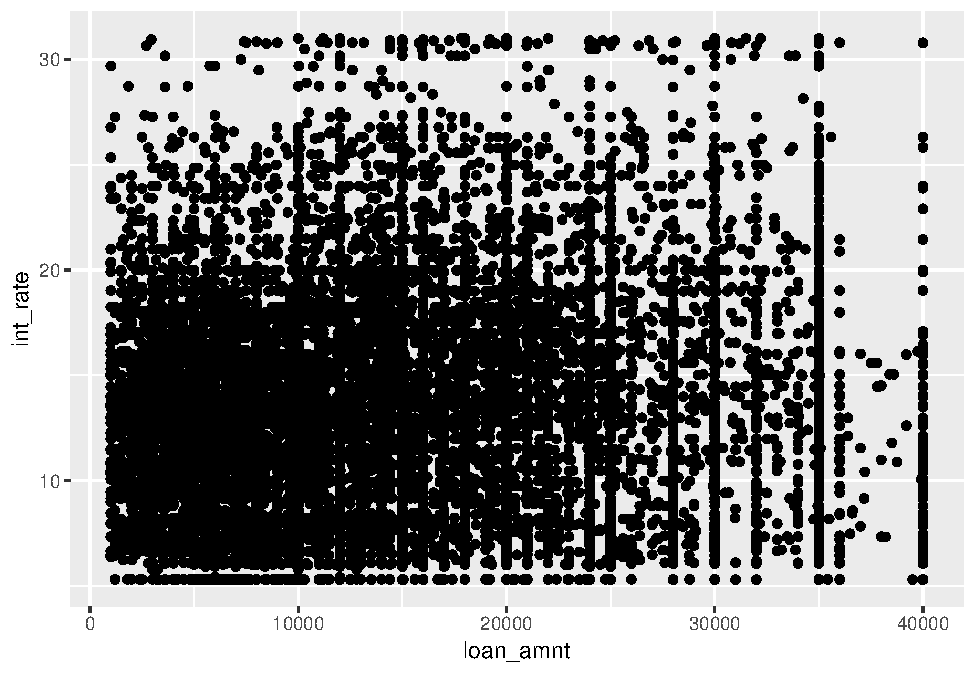
\includegraphics{Machine_learning_Group_7_files/figure-latex/Data Exploration - interest rate vs loan amount-1.pdf}

\begin{Shaded}
\begin{Highlighting}[]
\CommentTok{# from this visualisation we can't see any clear correlation.}
\end{Highlighting}
\end{Shaded}

\begin{Shaded}
\begin{Highlighting}[]
\CommentTok{# plotting the loan amount vs the term}
\NormalTok{\{}\KeywordTok{ggplot}\NormalTok{(}\DataTypeTok{data =}\NormalTok{ dataset_reg, }\DataTypeTok{mapping =} \KeywordTok{aes}\NormalTok{(term, int_rate)) }\OperatorTok{+}
\StringTok{  }\KeywordTok{geom_boxplot}\NormalTok{()\}}
\end{Highlighting}
\end{Shaded}

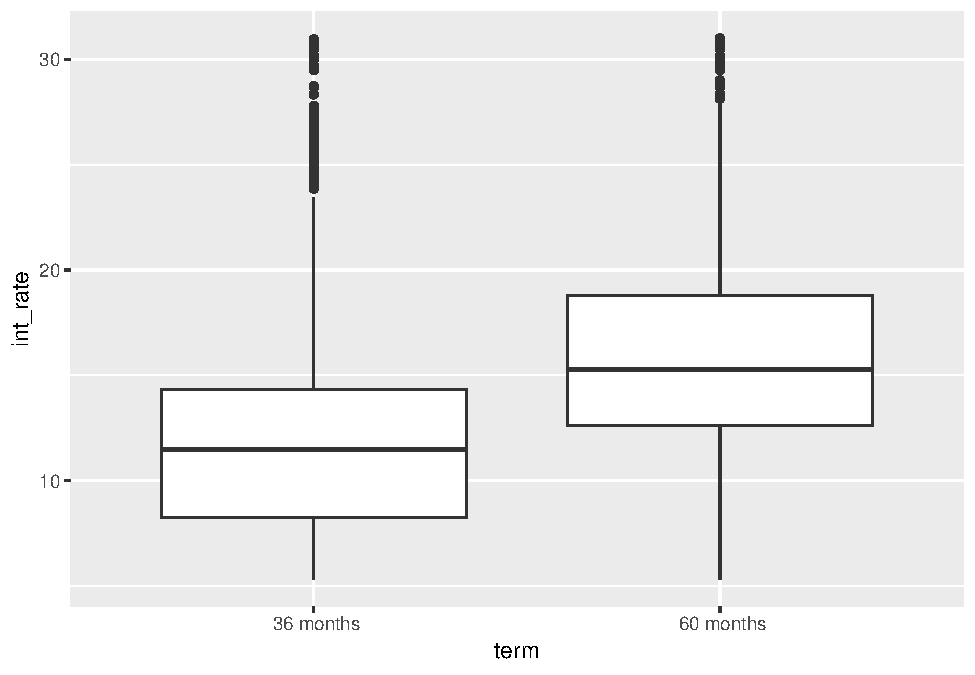
\includegraphics{Machine_learning_Group_7_files/figure-latex/Data Exploration - interest rate vs term-1.pdf}

\begin{Shaded}
\begin{Highlighting}[]
\CommentTok{# Here we can see that the interest rate is generaly higher for 60 months loans and lower for 36 months loans.}
\end{Highlighting}
\end{Shaded}

\begin{Shaded}
\begin{Highlighting}[]
\CommentTok{# plotting the loan amount vs the grade}
\NormalTok{\{}\KeywordTok{ggplot}\NormalTok{(}\DataTypeTok{data =}\NormalTok{ dataset_reg, }\DataTypeTok{mapping =} \KeywordTok{aes}\NormalTok{(}\KeywordTok{factor}\NormalTok{(sub_grade), int_rate), }\DataTypeTok{group =} \DecValTok{2}\NormalTok{) }\OperatorTok{+}
\StringTok{  }\KeywordTok{geom_boxplot}\NormalTok{()\}}
\end{Highlighting}
\end{Shaded}

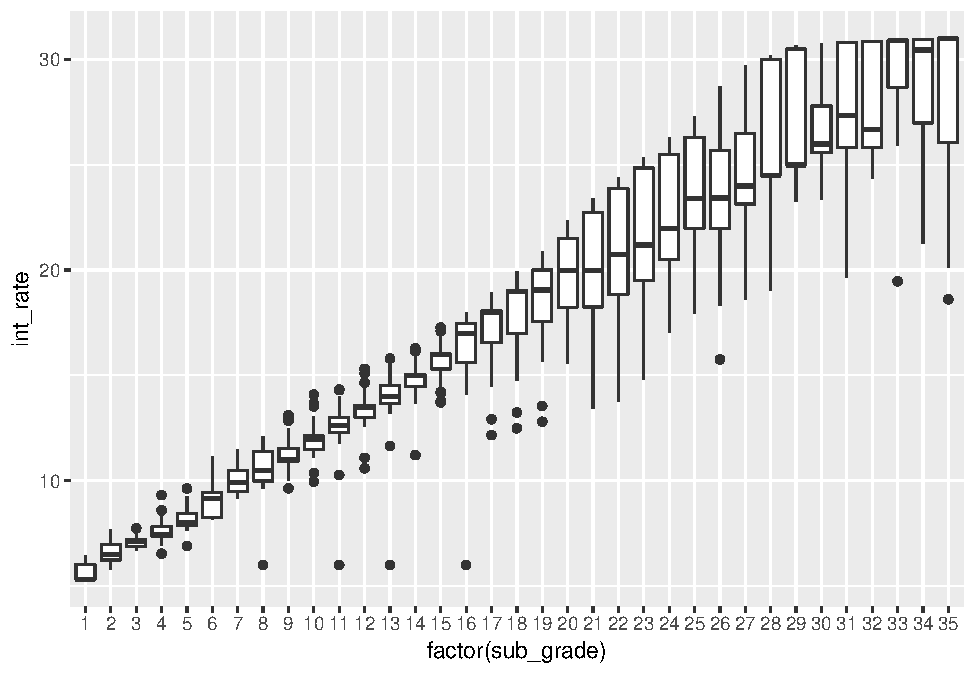
\includegraphics{Machine_learning_Group_7_files/figure-latex/Data Exploration - interest rate vs grade-1.pdf}

\begin{Shaded}
\begin{Highlighting}[]
\CommentTok{# The sub_grade seems to have a strong correlation with the interest rate}
\end{Highlighting}
\end{Shaded}

\begin{Shaded}
\begin{Highlighting}[]
\CommentTok{# plotting the loan amount vs home ownership}
\NormalTok{\{}\KeywordTok{ggplot}\NormalTok{(}\DataTypeTok{data =}\NormalTok{ dataset_reg, }\DataTypeTok{mapping =} \KeywordTok{aes}\NormalTok{(}\KeywordTok{factor}\NormalTok{(home_ownership), int_rate), }\DataTypeTok{group =} \DecValTok{2}\NormalTok{) }\OperatorTok{+}
\StringTok{  }\KeywordTok{geom_boxplot}\NormalTok{()\}}
\end{Highlighting}
\end{Shaded}

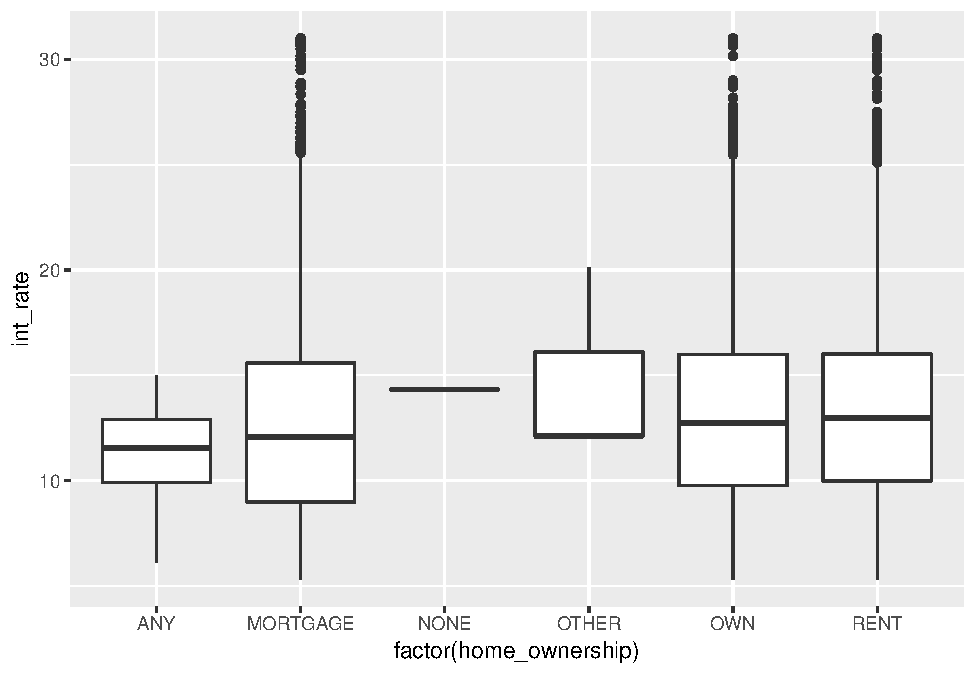
\includegraphics{Machine_learning_Group_7_files/figure-latex/Data Exploration - interest rate vs home ownership-1.pdf}

\begin{Shaded}
\begin{Highlighting}[]
\CommentTok{# Here we can see that the interest rate is quite close to each other between home_ownership.}
\end{Highlighting}
\end{Shaded}

\begin{Shaded}
\begin{Highlighting}[]
\CommentTok{# plotting the loan amount vs verification_status}
\NormalTok{\{}\KeywordTok{ggplot}\NormalTok{(}\DataTypeTok{data =}\NormalTok{ dataset_reg, }\DataTypeTok{mapping =} \KeywordTok{aes}\NormalTok{(}\KeywordTok{factor}\NormalTok{(verification_status), int_rate), }\DataTypeTok{group =} \DecValTok{2}\NormalTok{) }\OperatorTok{+}
\StringTok{  }\KeywordTok{geom_boxplot}\NormalTok{()\}}
\end{Highlighting}
\end{Shaded}

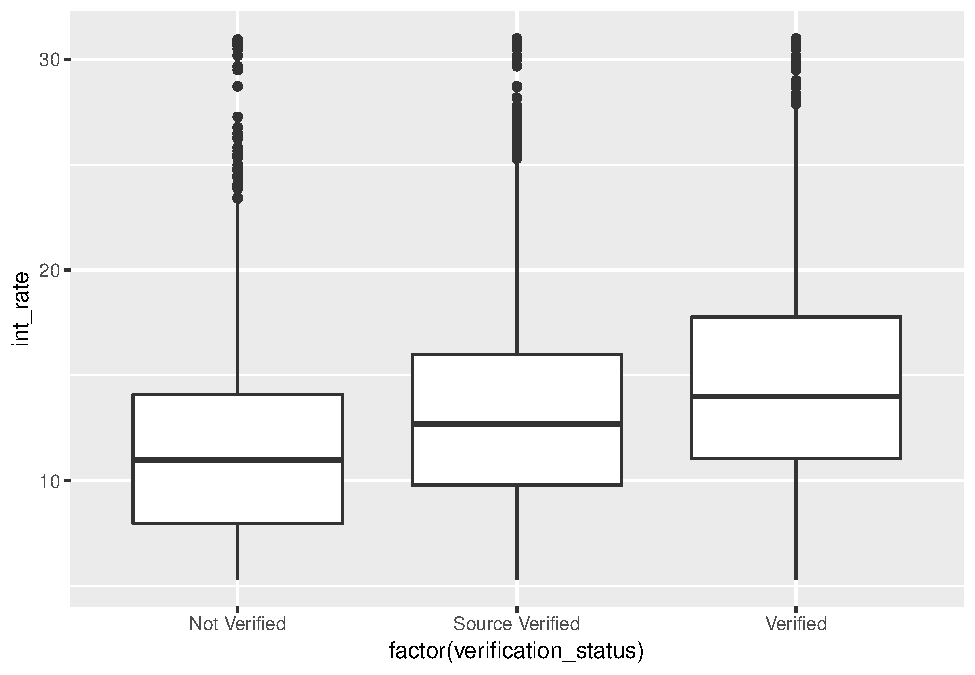
\includegraphics{Machine_learning_Group_7_files/figure-latex/Data Exploration - interest rate vs verification_status-1.pdf}

\begin{Shaded}
\begin{Highlighting}[]
\CommentTok{# The verification_status seems to also have an correlation with the interest rate.}
\end{Highlighting}
\end{Shaded}

\begin{Shaded}
\begin{Highlighting}[]
\CommentTok{# lm on the whole dataset_reg}
\NormalTok{lmp.fit=}\KeywordTok{lm}\NormalTok{(int_rate}\OperatorTok{~}\NormalTok{.,}\DataTypeTok{data =}\NormalTok{ dataset_reg)}

\KeywordTok{summary}\NormalTok{(lmp.fit)}
\KeywordTok{plot}\NormalTok{(lmp.fit)}
\CommentTok{#removing features that do not have at least a 0.001 P value}
\NormalTok{dataset_reg <-}\StringTok{ }\KeywordTok{subset}\NormalTok{(dataset_reg, }\DataTypeTok{select =} \OperatorTok{-}\KeywordTok{c}\NormalTok{(annual_inc, dti, earliest_cr_line,total_pymnt, total_rec_prncp, total_rec_int, total_rec_late_fee, recoveries, acc_open_past_24mths, avg_cur_bal, bc_open_to_buy, delinq_amnt, mo_sin_old_rev_tl_op, mo_sin_rcnt_rev_tl_op, mort_acc, num_il_tl, pct_tl_nvr_dlq, tax_liens, total_bal_ex_mort, total_bc_limit, total_il_high_credit_limit, num_actv_bc_tl, mo_sin_rcnt_tl))}

\CommentTok{# Doing a second round to see if further variables can be removed.}
\KeywordTok{summary}\NormalTok{(lmp.fit)}
\NormalTok{lmp.fit=}\KeywordTok{lm}\NormalTok{(int_rate}\OperatorTok{~}\NormalTok{.,}\DataTypeTok{data =}\NormalTok{ dataset_reg)}

\CommentTok{#removing features that do not have at least a 0.001 P value}

\NormalTok{dataset_reg <-}\StringTok{ }\KeywordTok{subset}\NormalTok{(dataset_reg, }\DataTypeTok{select =} \OperatorTok{-}\KeywordTok{c}\NormalTok{(hardship_reason, inq_last_6mths, num_actv_rev_tl, percent_bc_gt_}\DecValTok{75}\NormalTok{, tot_hi_cred_lim))}
                  
\NormalTok{lmp.fit=}\KeywordTok{lm}\NormalTok{(int_rate}\OperatorTok{~}\NormalTok{.,}\DataTypeTok{data =}\NormalTok{ dataset_reg)}
\KeywordTok{summary}\NormalTok{(lmp.fit)}

\NormalTok{dataset_reg <-}\StringTok{ }\KeywordTok{subset}\NormalTok{(dataset_reg, }\DataTypeTok{select =} \OperatorTok{-}\KeywordTok{c}\NormalTok{(bc_util))}
\end{Highlighting}
\end{Shaded}

\pagebreak

\hypertarget{main-task}{%
\subsection{Main task:}\label{main-task}}

\hypertarget{compare-three-different-methods-to-perform-regression-using-the-cross-validation-method-to-compute-the-best-parameters.-consider-using-some-regularization-for-the-parameters-shrinkage.-test-the-train-error-rate-the-cv-error-rate-and-the-test-error.}{%
\subsubsection{Compare three different methods to perform regression,
using the cross-validation method to compute the best parameters.
Consider using some regularization for the parameters shrinkage. Test
the train error rate, the CV error rate and the test
error.}\label{compare-three-different-methods-to-perform-regression-using-the-cross-validation-method-to-compute-the-best-parameters.-consider-using-some-regularization-for-the-parameters-shrinkage.-test-the-train-error-rate-the-cv-error-rate-and-the-test-error.}}

Stepwise Feature selection

\begin{Shaded}
\begin{Highlighting}[]
\CommentTok{## Read Model from file or compute it }
\ControlFlowTok{if}\NormalTok{ (}\KeywordTok{file.exists}\NormalTok{(}\StringTok{"fit.glmStepAIC.reg.rds"}\NormalTok{)) \{}
\NormalTok{   fit.bridge.reg <-}\StringTok{ }\KeywordTok{readRDS}\NormalTok{(}\StringTok{"fit.glmStepAIC.reg.rds"}\NormalTok{)}
\NormalTok{\} }\ControlFlowTok{else}\NormalTok{ \{}
\NormalTok{    fit.glmStepAIC.reg <-}\StringTok{ }\KeywordTok{train}\NormalTok{(int_rate}\OperatorTok{~}\NormalTok{.,}
                    \DataTypeTok{data =}\NormalTok{ dataset_reg,}
                    \DataTypeTok{method =} \StringTok{"glmStepAIC"}\NormalTok{,}
                    \DataTypeTok{na.action =}\NormalTok{ na.pass)}
\NormalTok{\}}
\NormalTok{fit.glmStepAIC.reg}
\NormalTok{fit.glmStepAIC.reg}\OperatorTok{$}\NormalTok{finalModel}
\KeywordTok{plot}\NormalTok{(fit.glmStepAIC.reg}\OperatorTok{$}\NormalTok{finalModel)}
\end{Highlighting}
\end{Shaded}

Limit the dataset by stepwise feature selection

\begin{Shaded}
\begin{Highlighting}[]
\NormalTok{dataset_reg <-}\StringTok{ }\KeywordTok{subset}\NormalTok{(dataset_reg, }\DataTypeTok{select =} \KeywordTok{c}\NormalTok{(int_rate, bc_util, delinq_2yrs, installment, initial_list_status, loan_status, revol_util, sub_grade))}
\end{Highlighting}
\end{Shaded}

\hypertarget{apply-the-validation-set-approach-to-reserve-a-meaningful-amount-of-data-for-the-test-phase.}{%
\subsubsection{Apply the ``validation set approach'' to reserve a
meaningful amount of data for the test
phase.}\label{apply-the-validation-set-approach-to-reserve-a-meaningful-amount-of-data-for-the-test-phase.}}

\begin{Shaded}
\begin{Highlighting}[]
\CommentTok{# setting a seed for reproducability}
\KeywordTok{set.seed}\NormalTok{(}\DecValTok{7}\NormalTok{)}
\CommentTok{# We randomly split our dataframe in a train and test set}
\NormalTok{trainRows =}\StringTok{ }\KeywordTok{sample}\NormalTok{(}\DecValTok{1}\OperatorTok{:}\KeywordTok{nrow}\NormalTok{(dataset_reg),}\FloatTok{0.8}\OperatorTok{*}\KeywordTok{nrow}\NormalTok{(dataset_reg))}
\NormalTok{testRows =}\StringTok{ }\KeywordTok{nrow}\NormalTok{(dataset_reg) }\OperatorTok{-}\StringTok{ }\NormalTok{trainRows}
\NormalTok{train.data.reg =}\StringTok{ }\NormalTok{dataset_reg[trainRows,]}
\NormalTok{test.data.reg =}\StringTok{ }\NormalTok{dataset_reg[}\OperatorTok{-}\NormalTok{trainRows,]}
\end{Highlighting}
\end{Shaded}

\begin{Shaded}
\begin{Highlighting}[]
\NormalTok{control.reg <-}\StringTok{ }\KeywordTok{trainControl}\NormalTok{(}\DataTypeTok{method =} \StringTok{"repeatedcv"}\NormalTok{, }\DataTypeTok{number =} \DecValTok{10}\NormalTok{, }\DataTypeTok{repeats =} \DecValTok{3}\NormalTok{)}
\end{Highlighting}
\end{Shaded}

\begin{Shaded}
\begin{Highlighting}[]
\ControlFlowTok{if}\NormalTok{ (}\KeywordTok{file.exists}\NormalTok{(}\StringTok{"fit.lm.reg.rds"}\NormalTok{)) \{}
\NormalTok{   fit.lm.reg <-}\StringTok{ }\KeywordTok{readRDS}\NormalTok{(}\StringTok{"fit.lm.reg.rds"}\NormalTok{)}
\NormalTok{\} }\ControlFlowTok{else}\NormalTok{ \{}
\NormalTok{  fit.lm.reg <-}\StringTok{ }\KeywordTok{train}\NormalTok{(int_rate}\OperatorTok{~}\NormalTok{.,}
                      \DataTypeTok{data =}\NormalTok{ train.data.reg,}
                      \DataTypeTok{trControl =}\NormalTok{ control.reg,}
                      \DataTypeTok{method =} \StringTok{"lm"}\NormalTok{,}
                      \DataTypeTok{na.action =}\NormalTok{ na.pass,}
                      \DataTypeTok{preProc =} \KeywordTok{c}\NormalTok{(}\StringTok{"zv"}\NormalTok{,}\StringTok{"center"}\NormalTok{,}\StringTok{"scale"}\NormalTok{))  }
\NormalTok{\}}
\NormalTok{fit.lm.reg}
\end{Highlighting}
\end{Shaded}

\begin{verbatim}
## Linear Regression 
## 
## 1600 samples
##    7 predictor
## 
## Pre-processing: centered (13), scaled (13), remove (1) 
## Resampling: Cross-Validated (10 fold, repeated 3 times) 
## Summary of sample sizes: 1440, 1440, 1439, 1440, 1440, 1440, ... 
## Resampling results:
## 
##   RMSE       Rsquared   MAE      
##   0.9786347  0.9562666  0.7197813
## 
## Tuning parameter 'intercept' was held constant at a value of TRUE
\end{verbatim}

\begin{Shaded}
\begin{Highlighting}[]
\NormalTok{fit.lm.reg}\OperatorTok{$}\NormalTok{finalModel}
\end{Highlighting}
\end{Shaded}

\begin{verbatim}
## 
## Call:
## lm(formula = .outcome ~ ., data = dat)
## 
## Coefficients:
##                                                      (Intercept)  
##                                                       12.9413125  
##                                                          bc_util  
##                                                        0.0574986  
##                                                      delinq_2yrs  
##                                                       -0.0488102  
##                                                      installment  
##                                                        0.0003816  
##                                             initial_list_statusw  
##                                                       -0.0616466  
##                                               loan_statusCurrent  
##                                                        0.2977986  
## `loan_statusDoes not meet the credit policy. Status:Charged Off`  
##                                                       -0.0908909  
##  `loan_statusDoes not meet the credit policy. Status:Fully Paid`  
##                                                       -0.1262483  
##                                          `loan_statusFully Paid`  
##                                                        0.1336417  
##                                     `loan_statusIn Grace Period`  
##                                                        0.0274737  
##                                   `loan_statusLate (16-30 days)`  
##                                                        0.0161922  
##                                  `loan_statusLate (31-120 days)`  
##                                                        0.0557831  
##                                                       revol_util  
##                                                       -0.0591781  
##                                                        sub_grade  
##                                                        4.5862552
\end{verbatim}

\begin{Shaded}
\begin{Highlighting}[]
\KeywordTok{plot}\NormalTok{(fit.lm.reg}\OperatorTok{$}\NormalTok{finalModel)}
\end{Highlighting}
\end{Shaded}

\begin{verbatim}
## Warning: not plotting observations with leverage one:
##   913, 1377
\end{verbatim}

\includegraphics{Machine_learning_Group_7_files/figure-latex/Linear Model analysis regression-1.pdf}
\includegraphics{Machine_learning_Group_7_files/figure-latex/Linear Model analysis regression-2.pdf}

\begin{verbatim}
## Warning: not plotting observations with leverage one:
##   913, 1377
\end{verbatim}

\includegraphics{Machine_learning_Group_7_files/figure-latex/Linear Model analysis regression-3.pdf}
\includegraphics{Machine_learning_Group_7_files/figure-latex/Linear Model analysis regression-4.pdf}

Fit the a extreme gradient boosting model.

\begin{Shaded}
\begin{Highlighting}[]
\ControlFlowTok{if}\NormalTok{ (}\KeywordTok{file.exists}\NormalTok{(}\StringTok{"fit.egb.reg.rds"}\NormalTok{)) \{}
\NormalTok{   fit.egb.reg <-}\StringTok{ }\KeywordTok{readRDS}\NormalTok{(}\StringTok{"fit.egb.reg.rds"}\NormalTok{)}
\NormalTok{\} }\ControlFlowTok{else}\NormalTok{ \{}
\NormalTok{    fit.egb.reg =}\StringTok{ }\KeywordTok{train}\NormalTok{(int_rate}\OperatorTok{~}\NormalTok{.,}
                    \DataTypeTok{data =}\NormalTok{ train.data.reg,}
                    \DataTypeTok{trControl =}\NormalTok{ control.reg,}
                    \DataTypeTok{method =} \StringTok{"xgbTree"}
\NormalTok{    )}
\NormalTok{\}}
\end{Highlighting}
\end{Shaded}

Fit the random forest model.

\begin{Shaded}
\begin{Highlighting}[]
\CommentTok{## Read Model from file or compute it }
\ControlFlowTok{if}\NormalTok{ (}\KeywordTok{file.exists}\NormalTok{(}\StringTok{"fit.RF.reg.rds"}\NormalTok{)) \{}
\NormalTok{   fit.RF.reg <-}\StringTok{ }\KeywordTok{readRDS}\NormalTok{(}\StringTok{"fit.RF.reg.rds"}\NormalTok{)}
\NormalTok{\} }\ControlFlowTok{else}\NormalTok{ \{}
\NormalTok{   fit.RF.reg <-}\StringTok{ }\KeywordTok{train}\NormalTok{(int_rate}\OperatorTok{~}\NormalTok{.,}
                    \DataTypeTok{data =}\NormalTok{ train.data.reg,}
                    \DataTypeTok{trControl =}\NormalTok{ control.reg,}
                    \DataTypeTok{method =} \StringTok{"parRF"}\NormalTok{,}
                    \DataTypeTok{na.action =}\NormalTok{ na.pass)}
\NormalTok{\}}

\NormalTok{fit.RF.reg}
\end{Highlighting}
\end{Shaded}

\begin{verbatim}
## Parallel Random Forest 
## 
## 10000 samples
##     7 predictor
## 
## No pre-processing
## Resampling: Cross-Validated (10 fold, repeated 3 times) 
## Summary of sample sizes: 8999, 9000, 8999, 9001, 9000, 9001, ... 
## Resampling results across tuning parameters:
## 
##   mtry  RMSE       Rsquared   MAE      
##    2    2.5657588  0.8720705  1.8120652
##    8    0.9199010  0.9640665  0.6358753
##   14    0.9321221  0.9630738  0.6342602
## 
## RMSE was used to select the optimal model using the smallest value.
## The final value used for the model was mtry = 8.
\end{verbatim}

\begin{Shaded}
\begin{Highlighting}[]
\NormalTok{fit.RF.reg}\OperatorTok{$}\NormalTok{finalModel}
\end{Highlighting}
\end{Shaded}

\begin{verbatim}
## 
## Call:
##  randomForest(x = "x", y = "y", ntree = 125, mtry = 8) 
##                Type of random forest: regression
##                      Number of trees: 500
## No. of variables tried at each split: 8
\end{verbatim}

\begin{Shaded}
\begin{Highlighting}[]
\KeywordTok{plot}\NormalTok{(fit.RF.reg)}
\end{Highlighting}
\end{Shaded}

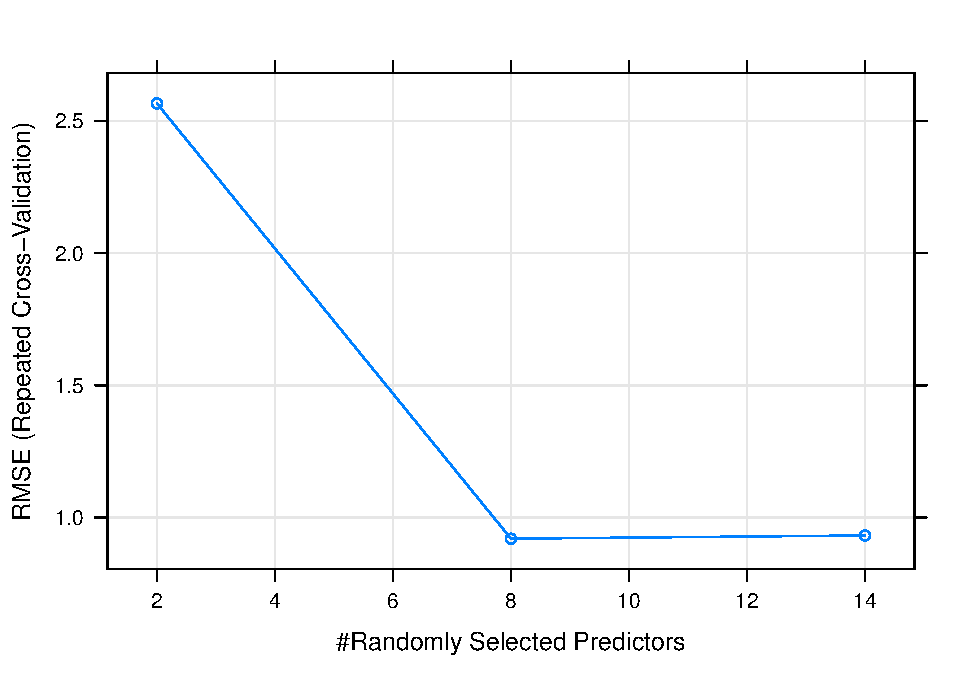
\includegraphics{Machine_learning_Group_7_files/figure-latex/Random Forest-1.pdf}

\begin{Shaded}
\begin{Highlighting}[]
\CommentTok{# MAPE LM }\AlertTok{TEST}
\NormalTok{mape_lm_test <-}\StringTok{ }\KeywordTok{MAPE}\NormalTok{(}\KeywordTok{predict}\NormalTok{(fit.lm.reg, test.data.reg), test.data.reg}\OperatorTok{$}\NormalTok{int_rate)}

\CommentTok{# MAPE ExtremGradiantBoosting }\AlertTok{TEST}
\NormalTok{mape_egb_test <-}\StringTok{ }\KeywordTok{MAPE}\NormalTok{(}\KeywordTok{predict}\NormalTok{(fit.egb.reg, test.data.reg), test.data.reg}\OperatorTok{$}\NormalTok{int_rate)}

\CommentTok{# MAPE Random Forest }\AlertTok{TEST}
\NormalTok{mape_rf_test <-}\StringTok{ }\KeywordTok{MAPE}\NormalTok{(}\KeywordTok{predict}\NormalTok{(fit.RF.reg, test.data.reg), test.data.reg}\OperatorTok{$}\NormalTok{int_rate)}

\NormalTok{test_mapes <-}\StringTok{ }\KeywordTok{data.frame}\NormalTok{(}\StringTok{"LM"}\NormalTok{ =}\StringTok{ }\NormalTok{mape_lm_test, }\StringTok{"egb"}\NormalTok{=}\StringTok{ }\NormalTok{mape_egb_test, }\StringTok{"Random Forest"}\NormalTok{ =}\StringTok{ }\NormalTok{mape_rf_test)}
\end{Highlighting}
\end{Shaded}

\begin{Shaded}
\begin{Highlighting}[]
\CommentTok{# MAPE LM train}
\NormalTok{mape_lm_train <-}\StringTok{ }\KeywordTok{MAPE}\NormalTok{(}\KeywordTok{predict}\NormalTok{(fit.lm.reg, train.data.reg), train.data.reg}\OperatorTok{$}\NormalTok{int_rate)}

\CommentTok{# MAPE ExtremGradiantBoosting train}
\NormalTok{mape_egb_train <-}\StringTok{ }\KeywordTok{MAPE}\NormalTok{(}\KeywordTok{predict}\NormalTok{(fit.egb.reg, train.data.reg), train.data.reg}\OperatorTok{$}\NormalTok{int_rate)}

\CommentTok{# MAPE Randdom Forest train}
\NormalTok{mape_rf_train <-}\StringTok{ }\KeywordTok{MAPE}\NormalTok{(}\KeywordTok{predict}\NormalTok{(fit.RF.reg, train.data.reg), train.data.reg}\OperatorTok{$}\NormalTok{int_rate)}

\NormalTok{train_mapes <-}\StringTok{ }\KeywordTok{data.frame}\NormalTok{(}\StringTok{"LM"}\NormalTok{ =}\StringTok{ }\NormalTok{mape_lm_train, }\StringTok{"egb"}\NormalTok{=}\StringTok{ }\NormalTok{mape_egb_train, }\StringTok{"Random Forest"}\NormalTok{ =}\StringTok{ }\NormalTok{mape_rf_train)}
\end{Highlighting}
\end{Shaded}

\begin{Shaded}
\begin{Highlighting}[]
\CommentTok{# Grouping Test and Train MAPEs}
\NormalTok{mapes <-}\StringTok{ }\KeywordTok{union}\NormalTok{(test_mapes, train_mapes)}
\KeywordTok{row.names}\NormalTok{(mapes) <-}\StringTok{ }\KeywordTok{c}\NormalTok{(}\StringTok{"test"}\NormalTok{, }\StringTok{"train"}\NormalTok{)}
\KeywordTok{print}\NormalTok{(mapes)}
\end{Highlighting}
\end{Shaded}

\begin{verbatim}
##               LM        egb Random.Forest
## test  0.05465464 0.05131145    0.04796991
## train 0.05259790 0.04917651    0.03103895
\end{verbatim}

\pagebreak

\hypertarget{part-2---classification-analysis}{%
\section{Part 2 - Classification
Analysis}\label{part-2---classification-analysis}}

Our goal in the second part of the assignment is to predict if a new
customer will be able to fully pay back their loans using a
classification method. Thus, we concentrate on the ``concluded lends''
in the data set, i.e., on all lends whose loan\_status is not Current.

\hypertarget{preparatory-tasks-1}{%
\subsection{Preparatory tasks}\label{preparatory-tasks-1}}

We filter out all observations with loan\_status == Current. For the
remaining observations, we check if the loan\_status is ``Fully Paid''.
If not, change the value of loan\_status to ``DEFAULTED''.

\begin{Shaded}
\begin{Highlighting}[]
\CommentTok{# set dataset as data.table::datatable}
\KeywordTok{setDT}\NormalTok{(dataset)}

\CommentTok{# filter out all observations with loan_status == Current and storing it in a separate Data}
\NormalTok{dataset_cla <-}\StringTok{ }\NormalTok{dataset[loan_status }\OperatorTok{!=}\StringTok{ 'Current'}\NormalTok{]}

\CommentTok{# change all the loan status that are not "Fully Paid" to 1}
\NormalTok{dataset_cla}\OperatorTok{$}\NormalTok{defaulted[dataset_cla}\OperatorTok{$}\NormalTok{loan_status }\OperatorTok{!=}\StringTok{ "Fully Paid"}\NormalTok{] <-}\StringTok{ }\DecValTok{1}

\CommentTok{# change level of defaulted to 1 and 0 }
\KeywordTok{levels}\NormalTok{(dataset_cla}\OperatorTok{$}\NormalTok{defaulted) =}\StringTok{ }\KeywordTok{c}\NormalTok{(}\DecValTok{1}\NormalTok{, }\DecValTok{0}\NormalTok{)}

\CommentTok{# Change all the defaulted values that aren't "Default" to 0}
\NormalTok{dataset_cla}\OperatorTok{$}\NormalTok{defaulted[}\KeywordTok{is.na}\NormalTok{(dataset_cla}\OperatorTok{$}\NormalTok{defaulted)] <-}\StringTok{ }\DecValTok{0}

\CommentTok{# remove origin variable, because defaulted is relevant now}
\NormalTok{dataset_cla}\OperatorTok{$}\NormalTok{loan_status <-}\StringTok{ }\OtherTok{NULL}

\CommentTok{# set defaulted as factor}
\NormalTok{dataset_cla}\OperatorTok{$}\NormalTok{defaulted <-}\StringTok{ }\KeywordTok{as.factor}\NormalTok{(dataset_cla}\OperatorTok{$}\NormalTok{defaulted)}

\CommentTok{# confirm steps below, by checking results}
\KeywordTok{table}\NormalTok{(dataset_cla}\OperatorTok{$}\NormalTok{defaulted)}
\end{Highlighting}
\end{Shaded}

\begin{verbatim}
## 
##    0    1 
## 9205 2670
\end{verbatim}

\hypertarget{create-a-validation-set.}{%
\subsubsection{Create a validation
set.}\label{create-a-validation-set.}}

\begin{Shaded}
\begin{Highlighting}[]
\CommentTok{# setting a seed for reproducability}
\KeywordTok{set.seed}\NormalTok{(}\DecValTok{7}\NormalTok{)}

\CommentTok{# random split into  train and test set, with a ratio of 20:80}
\NormalTok{trainIndex <-}\StringTok{ }\KeywordTok{sample}\NormalTok{(}\DecValTok{1}\OperatorTok{:}\KeywordTok{nrow}\NormalTok{(dataset_cla),}\FloatTok{0.8}\OperatorTok{*}\KeywordTok{nrow}\NormalTok{(dataset_cla))}

\NormalTok{train.data.cla <-}\StringTok{ }\NormalTok{dataset_cla[trainIndex,]}
\NormalTok{test.data.cla  <-}\StringTok{ }\NormalTok{dataset_cla[}\OperatorTok{-}\NormalTok{trainIndex,]}
\end{Highlighting}
\end{Shaded}

\hypertarget{data-exploration-1}{%
\subsection{Data Exploration}\label{data-exploration-1}}

\begin{Shaded}
\begin{Highlighting}[]
\NormalTok{\{}\KeywordTok{ggplot}\NormalTok{(}\DataTypeTok{data =}\NormalTok{ dataset_cla, }\DataTypeTok{mapping =} \KeywordTok{aes}\NormalTok{(defaulted, int_rate)) }\OperatorTok{+}
\StringTok{    }\KeywordTok{geom_boxplot}\NormalTok{()\}}
\end{Highlighting}
\end{Shaded}

\includegraphics{Machine_learning_Group_7_files/figure-latex/Data Exploration Classification defaulted int_rate-1.pdf}

\begin{Shaded}
\begin{Highlighting}[]
\CommentTok{# We can see that credits who defaulted generally have a higher int_rate}
\end{Highlighting}
\end{Shaded}

\hypertarget{main-tasks}{%
\subsection{Main tasks:}\label{main-tasks}}

Now we can go over to do the analysis on the dataset. Therefore we use
different approaches for feature selection (PLS and PCA). Based on the
results, we choose the features and do the classification analysis.

\hypertarget{use-principal-component-analysis-for-base-transformation-and-then-compare-it-with-the-partial-least-squares-regression-result.-select-the-best-base-with-cross-validation-using-the-better-of-the-two-approaches.}{%
\subsubsection{Use Principal Component Analysis for base transformation
and then compare it with the Partial Least Squares Regression result.
Select the best base with cross validation, using the better of the two
approaches.}\label{use-principal-component-analysis-for-base-transformation-and-then-compare-it-with-the-partial-least-squares-regression-result.-select-the-best-base-with-cross-validation-using-the-better-of-the-two-approaches.}}

\begin{Shaded}
\begin{Highlighting}[]
\CommentTok{# Compile cross-validation settings}
\KeywordTok{set.seed}\NormalTok{(}\DecValTok{100}\NormalTok{)}
\NormalTok{myfolds.cla <-}\StringTok{ }\KeywordTok{createMultiFolds}\NormalTok{(train.data.cla, }\DataTypeTok{k =} \DecValTok{5}\NormalTok{, }\DataTypeTok{times =} \DecValTok{10}\NormalTok{)}
\NormalTok{control.cla <-}\StringTok{ }\KeywordTok{trainControl}\NormalTok{(}\StringTok{"repeatedcv"}\NormalTok{, }\DataTypeTok{index =}\NormalTok{ myfolds.cla, }\DataTypeTok{selectionFunction =} \StringTok{"oneSE"}\NormalTok{)}
\end{Highlighting}
\end{Shaded}

Perform Partial Least Squares Regression with caret package, to have a
standartized handling.

\begin{Shaded}
\begin{Highlighting}[]
\CommentTok{# Train PLS model}
\NormalTok{fit.pls.cla <-}\StringTok{ }\KeywordTok{train}\NormalTok{(defaulted }\OperatorTok{~}\StringTok{ }\NormalTok{., }\DataTypeTok{data =}\NormalTok{ train.data.cla,}
 \DataTypeTok{method =} \StringTok{"pls"}\NormalTok{,}
 \DataTypeTok{metric =} \StringTok{"Accuracy"}\NormalTok{,}
 \DataTypeTok{tuneLength =} \DecValTok{20}\NormalTok{,}
 \DataTypeTok{trControl =}\NormalTok{ control.cla,}
 \DataTypeTok{preProc =} \KeywordTok{c}\NormalTok{(}\StringTok{"zv"}\NormalTok{,}\StringTok{"center"}\NormalTok{,}\StringTok{"scale"}\NormalTok{))}

\KeywordTok{plot}\NormalTok{(fit.pls.cla)}
\end{Highlighting}
\end{Shaded}

\includegraphics{Machine_learning_Group_7_files/figure-latex/PLS analysis-1.pdf}

Perform Principal Component Analysis with caret package, to have a
standartized handling.

\begin{Shaded}
\begin{Highlighting}[]
\CommentTok{# PCA-DA}
\NormalTok{fit.lda.cla <-}\StringTok{ }\KeywordTok{train}\NormalTok{(defaulted }\OperatorTok{~}\StringTok{ }\NormalTok{., }\DataTypeTok{data =}\NormalTok{ train.data.cla,}
\DataTypeTok{method =} \StringTok{"lda"}\NormalTok{,}
\DataTypeTok{metric =} \StringTok{"Accuracy"}\NormalTok{,}
\DataTypeTok{trControl =}\NormalTok{ control.cla,}
\DataTypeTok{preProc =} \KeywordTok{c}\NormalTok{(}\StringTok{"zv"}\NormalTok{,}\StringTok{"center"}\NormalTok{,}\StringTok{"scale"}\NormalTok{,}\StringTok{"pca"}\NormalTok{))}
\end{Highlighting}
\end{Shaded}

Compile models and compare performance

\begin{Shaded}
\begin{Highlighting}[]
\NormalTok{models <-}\StringTok{ }\KeywordTok{resamples}\NormalTok{(}\KeywordTok{list}\NormalTok{(}\StringTok{"PLS-DA"}\NormalTok{ =}\StringTok{ }\NormalTok{fit.pls.cla, }\StringTok{"PCA-DA"}\NormalTok{ =}\StringTok{ }\NormalTok{fit.lda.cla))}
\KeywordTok{bwplot}\NormalTok{(models, }\DataTypeTok{metric =} \StringTok{"Accuracy"}\NormalTok{)}
\end{Highlighting}
\end{Shaded}

\includegraphics{Machine_learning_Group_7_files/figure-latex/unnamed-chunk-5-1.pdf}

\begin{Shaded}
\begin{Highlighting}[]
\KeywordTok{plot}\NormalTok{(}\KeywordTok{varImp}\NormalTok{(fit.pls.cla), fit.pls.cla}\OperatorTok{$}\NormalTok{bestTune}\OperatorTok{$}\NormalTok{ncomp, }\DataTypeTok{main =} \StringTok{"PLS-DA"}\NormalTok{)}
\end{Highlighting}
\end{Shaded}

\includegraphics{Machine_learning_Group_7_files/figure-latex/unnamed-chunk-5-2.pdf}

\begin{Shaded}
\begin{Highlighting}[]
\CommentTok{# limiting the variables of the dataset based on the results from PLS analysis in the step before}

\NormalTok{train.data.cla <-}\StringTok{ }\KeywordTok{subset}\NormalTok{(train.data.cla, }\DataTypeTok{select =} \KeywordTok{c}\NormalTok{(defaulted, total_rec_prncp, recoveries, collection_recovery_fee, last_pymnt_amnt, total_pymnt_inv, total_pymnt, debt_settlement_flag, sub_grade, int_rate, out_prncp, out_prncp_inv, settlement_status, term))}
\NormalTok{test.data.cla  <-}\StringTok{ }\KeywordTok{subset}\NormalTok{(test.data.cla, }\DataTypeTok{select =} \KeywordTok{c}\NormalTok{(defaulted, total_rec_prncp, recoveries, collection_recovery_fee, last_pymnt_amnt, total_pymnt_inv, total_pymnt, debt_settlement_flag, sub_grade, int_rate, out_prncp, out_prncp_inv, settlement_status, term))}
\end{Highlighting}
\end{Shaded}

\hypertarget{perform-the-classification-using-knn-logistic-regression-decision-tree-and-random-forest.}{%
\subsubsection{Perform the classification using KNN, Logistic
Regression, Decision Tree and Random
Forest.}\label{perform-the-classification-using-knn-logistic-regression-decision-tree-and-random-forest.}}

Train a model with KNN

\begin{Shaded}
\begin{Highlighting}[]
\CommentTok{## knn}
\NormalTok{fit.knn.cla  <-}\StringTok{ }\KeywordTok{train}\NormalTok{(defaulted }\OperatorTok{~}\StringTok{ }\NormalTok{., }
                \DataTypeTok{data =}\NormalTok{ train.data.cla, }
                \DataTypeTok{method =} \StringTok{"knn"}\NormalTok{,}
                \DataTypeTok{trControl =}\NormalTok{ control.cla,}
                \DataTypeTok{preProc =} \KeywordTok{c}\NormalTok{(}\StringTok{"zv"}\NormalTok{,}\StringTok{"center"}\NormalTok{,}\StringTok{"scale"}\NormalTok{)}
\NormalTok{                ) }
\end{Highlighting}
\end{Shaded}

Train a model with Logistic Regression

\begin{Shaded}
\begin{Highlighting}[]
\CommentTok{## logistic regression}
\NormalTok{fit.lreg.cla <-}\KeywordTok{train}\NormalTok{(defaulted }\OperatorTok{~}\StringTok{ }\NormalTok{recoveries }\OperatorTok{+}\StringTok{ }\NormalTok{collection_recovery_fee }\OperatorTok{+}\StringTok{ }\NormalTok{total_rec_prncp }
\OperatorTok{+}\StringTok{ }\NormalTok{last_pymnt_amnt }\OperatorTok{+}\StringTok{ }\NormalTok{total_pymnt, }
                \DataTypeTok{data =}\NormalTok{ train.data.cla, }
                \DataTypeTok{method =} \StringTok{"glm"}\NormalTok{,}
                \DataTypeTok{trControl =}\NormalTok{ control.cla,}
                \DataTypeTok{family=}\KeywordTok{binomial}\NormalTok{(),}
                \DataTypeTok{preProc =} \KeywordTok{c}\NormalTok{(}\StringTok{"zv"}\NormalTok{,}\StringTok{"center"}\NormalTok{,}\StringTok{"scale"}\NormalTok{)}
\NormalTok{                ) }
\end{Highlighting}
\end{Shaded}

Train a model with Decision Trees

\begin{Shaded}
\begin{Highlighting}[]
\CommentTok{## decision tree }
\NormalTok{fit.dtree.cla <-}\KeywordTok{train}\NormalTok{(defaulted }\OperatorTok{~}\StringTok{ }\NormalTok{recoveries }\OperatorTok{+}\StringTok{ }\NormalTok{collection_recovery_fee }\OperatorTok{+}\StringTok{ }\NormalTok{total_rec_prncp }
\OperatorTok{+}\StringTok{ }\NormalTok{last_pymnt_amnt }\OperatorTok{+}\StringTok{ }\NormalTok{total_pymnt, }
               \DataTypeTok{data=}\NormalTok{train.data.cla,}
               \DataTypeTok{method=}\StringTok{"ctree"}\NormalTok{,}
               \DataTypeTok{trControl =}\NormalTok{ control.cla,}
               \DataTypeTok{preProc =} \KeywordTok{c}\NormalTok{(}\StringTok{"zv"}\NormalTok{,}\StringTok{"center"}\NormalTok{,}\StringTok{"scale"}\NormalTok{))}
\end{Highlighting}
\end{Shaded}

Train a model with Random Forest

\begin{Shaded}
\begin{Highlighting}[]
\CommentTok{## random forest }
\NormalTok{fit.rf.cla <-}\KeywordTok{train}\NormalTok{(defaulted }\OperatorTok{~}\StringTok{ }\NormalTok{recoveries }\OperatorTok{+}\StringTok{ }\NormalTok{collection_recovery_fee }\OperatorTok{+}\StringTok{ }\NormalTok{total_rec_prncp }
\OperatorTok{+}\StringTok{ }\NormalTok{last_pymnt_amnt }\OperatorTok{+}\StringTok{ }\NormalTok{total_pymnt, }
               \DataTypeTok{data=}\NormalTok{train.data.cla,}
               \DataTypeTok{method=}\StringTok{"rf"}\NormalTok{,}
               \DataTypeTok{trControl =}\NormalTok{ control.cla,}
               \DataTypeTok{preProc =} \KeywordTok{c}\NormalTok{(}\StringTok{"zv"}\NormalTok{,}\StringTok{"center"}\NormalTok{,}\StringTok{"scale"}\NormalTok{))}
\end{Highlighting}
\end{Shaded}

\hypertarget{compare-the-respective-train-and-test-error-performances-to-select-one-of-these-approaches.}{%
\subsubsection{Compare the respective train and test error performances
to select one of these
approaches.}\label{compare-the-respective-train-and-test-error-performances-to-select-one-of-these-approaches.}}

\begin{Shaded}
\begin{Highlighting}[]
\KeywordTok{par}\NormalTok{(}\DataTypeTok{pty =} \StringTok{"s"}\NormalTok{)}
\KeywordTok{roc}\NormalTok{(test.data.cla}\OperatorTok{$}\NormalTok{defaulted, }\KeywordTok{as.numeric}\NormalTok{(}\KeywordTok{predict}\NormalTok{(fit.dtree.cla, }
\NormalTok{test.data.cla)), }\DataTypeTok{plot=}\OtherTok{TRUE}\NormalTok{, }\DataTypeTok{legacy.axes=}\OtherTok{TRUE}\NormalTok{, }
    \DataTypeTok{percent=}\OtherTok{TRUE}\NormalTok{, }\DataTypeTok{xlab=}\StringTok{"False Positive Percentage"}\NormalTok{, }\DataTypeTok{ylab=}\StringTok{"True Postive Percentage"}\NormalTok{, }\DataTypeTok{col=}\StringTok{"#377eb8"}\NormalTok{, }
    \DataTypeTok{lwd=}\DecValTok{4}\NormalTok{, }\DataTypeTok{print.auc =} \OtherTok{TRUE}\NormalTok{, }\DataTypeTok{print.auc.y=}\DecValTok{80}\NormalTok{, }\DataTypeTok{print.auc.x=}\DecValTok{30}\NormalTok{)}
\end{Highlighting}
\end{Shaded}

\begin{verbatim}
## 
## Call:
## roc.default(response = test.data.cla$defaulted, predictor = as.numeric(predict(fit.dtree.cla,     test.data.cla)), percent = TRUE, plot = TRUE, legacy.axes = TRUE,     xlab = "False Positive Percentage", ylab = "True Postive Percentage",     col = "#377eb8", lwd = 4, print.auc = TRUE, print.auc.y = 80,     print.auc.x = 30)
## 
## Data: as.numeric(predict(fit.dtree.cla, test.data.cla)) in 1832 controls (test.data.cla$defaulted 0) < 543 cases (test.data.cla$defaulted 1).
## Area under the curve: 92.55%
\end{verbatim}

\begin{Shaded}
\begin{Highlighting}[]
\KeywordTok{plot.roc}\NormalTok{(test.data.cla}\OperatorTok{$}\NormalTok{defaulted, }\KeywordTok{as.numeric}\NormalTok{(}\KeywordTok{predict}\NormalTok{(fit.rf.cla, }
\NormalTok{test.data.cla)), }\DataTypeTok{percent=}\OtherTok{TRUE}\NormalTok{, }\DataTypeTok{col=}\StringTok{"#b8377e"}\NormalTok{, }
         \DataTypeTok{lwd=}\DecValTok{4}\NormalTok{, }\DataTypeTok{print.auc=}\OtherTok{TRUE}\NormalTok{, }\DataTypeTok{add=}\OtherTok{TRUE}\NormalTok{, }\DataTypeTok{print.auc.y=}\DecValTok{70}\NormalTok{, }\DataTypeTok{print.auc.x=}\DecValTok{30}\NormalTok{)}

\KeywordTok{plot.roc}\NormalTok{(test.data.cla}\OperatorTok{$}\NormalTok{defaulted, }\KeywordTok{as.numeric}\NormalTok{(}\KeywordTok{predict}\NormalTok{(fit.lreg.cla, test.data.cla)), }
         \DataTypeTok{percent=}\OtherTok{TRUE}\NormalTok{, }\DataTypeTok{col=}\StringTok{"#b87137"}\NormalTok{, }\DataTypeTok{lwd=}\DecValTok{4}\NormalTok{, }\DataTypeTok{print.auc=}\OtherTok{TRUE}\NormalTok{, }\DataTypeTok{add=}\OtherTok{TRUE}\NormalTok{, }\DataTypeTok{print.auc.y=}\DecValTok{60}\NormalTok{, }\DataTypeTok{print.auc.x=}\DecValTok{30}\NormalTok{)}

\KeywordTok{plot.roc}\NormalTok{(test.data.cla}\OperatorTok{$}\NormalTok{defaulted, }\KeywordTok{as.numeric}\NormalTok{(}\KeywordTok{predict}\NormalTok{(fit.knn.cla, test.data.cla)), }
         \DataTypeTok{percent=}\OtherTok{TRUE}\NormalTok{, }\DataTypeTok{col=}\StringTok{"#7eb837"}\NormalTok{, }\DataTypeTok{lwd=}\DecValTok{4}\NormalTok{, }\DataTypeTok{print.auc=}\OtherTok{TRUE}\NormalTok{, }\DataTypeTok{add=}\OtherTok{TRUE}\NormalTok{, }\DataTypeTok{print.auc.y=}\DecValTok{50}\NormalTok{, }\DataTypeTok{print.auc.x=}\DecValTok{30}\NormalTok{)}
    
    \KeywordTok{legend}\NormalTok{(}\StringTok{"bottomright"}\NormalTok{, }\DataTypeTok{legend=}\KeywordTok{c}\NormalTok{(}\StringTok{"Decission Tree"}\NormalTok{, }
    \StringTok{"Random Forest"}\NormalTok{, }\StringTok{"Logisitic Regression"}\NormalTok{, }\StringTok{"KNN"}\NormalTok{), }
    \DataTypeTok{col=}\KeywordTok{c}\NormalTok{(}\StringTok{"#377eb8"}\NormalTok{, }\StringTok{"#b8377e"}\NormalTok{, }\StringTok{"#b87137"}\NormalTok{, }\StringTok{"#7eb837"}\NormalTok{), }\DataTypeTok{lwd=}\DecValTok{4}\NormalTok{)}
\end{Highlighting}
\end{Shaded}

\includegraphics{Machine_learning_Group_7_files/figure-latex/ROC Plot-1.pdf}

\hypertarget{perform-the-prediction-on-the-validation-set-and-compute-the-confusion-matrix.}{%
\subsubsection{Perform the prediction on the validation set and compute
the confusion
matrix.}\label{perform-the-prediction-on-the-validation-set-and-compute-the-confusion-matrix.}}

\begin{Shaded}
\begin{Highlighting}[]
\CommentTok{#Confusion Matrix KNN}
\KeywordTok{confusionMatrix}\NormalTok{( }\KeywordTok{predict}\NormalTok{(fit.knn.cla, test.data.cla), test.data.cla}\OperatorTok{$}\NormalTok{defaulted)    }\CommentTok{#Test}
\end{Highlighting}
\end{Shaded}

\begin{verbatim}
## Confusion Matrix and Statistics
## 
##           Reference
## Prediction    0    1
##          0 1816  293
##          1   16  250
##                                           
##                Accuracy : 0.8699          
##                  95% CI : (0.8557, 0.8832)
##     No Information Rate : 0.7714          
##     P-Value [Acc > NIR] : < 2.2e-16       
##                                           
##                   Kappa : 0.5505          
##                                           
##  Mcnemar's Test P-Value : < 2.2e-16       
##                                           
##             Sensitivity : 0.9913          
##             Specificity : 0.4604          
##          Pos Pred Value : 0.8611          
##          Neg Pred Value : 0.9398          
##              Prevalence : 0.7714          
##          Detection Rate : 0.7646          
##    Detection Prevalence : 0.8880          
##       Balanced Accuracy : 0.7258          
##                                           
##        'Positive' Class : 0               
## 
\end{verbatim}

\begin{Shaded}
\begin{Highlighting}[]
\CommentTok{#Confusion Matrix Logistic Regression}
\KeywordTok{confusionMatrix}\NormalTok{( }\KeywordTok{predict}\NormalTok{(fit.lreg.cla, test.data.cla), test.data.cla}\OperatorTok{$}\NormalTok{defaulted)   }\CommentTok{#Test}
\end{Highlighting}
\end{Shaded}

\begin{verbatim}
## Confusion Matrix and Statistics
## 
##           Reference
## Prediction    0    1
##          0 1807   74
##          1   25  469
##                                          
##                Accuracy : 0.9583         
##                  95% CI : (0.9495, 0.966)
##     No Information Rate : 0.7714         
##     P-Value [Acc > NIR] : < 2.2e-16      
##                                          
##                   Kappa : 0.8779         
##                                          
##  Mcnemar's Test P-Value : 1.406e-06      
##                                          
##             Sensitivity : 0.9864         
##             Specificity : 0.8637         
##          Pos Pred Value : 0.9607         
##          Neg Pred Value : 0.9494         
##              Prevalence : 0.7714         
##          Detection Rate : 0.7608         
##    Detection Prevalence : 0.7920         
##       Balanced Accuracy : 0.9250         
##                                          
##        'Positive' Class : 0              
## 
\end{verbatim}

\begin{Shaded}
\begin{Highlighting}[]
\CommentTok{#Confusion Matrix Decision Trees}
\KeywordTok{confusionMatrix}\NormalTok{( }\KeywordTok{predict}\NormalTok{(fit.dtree.cla, test.data.cla), test.data.cla}\OperatorTok{$}\NormalTok{defaulted)  }\CommentTok{#Test}
\end{Highlighting}
\end{Shaded}

\begin{verbatim}
## Confusion Matrix and Statistics
## 
##           Reference
## Prediction    0    1
##          0 1819   77
##          1   13  466
##                                           
##                Accuracy : 0.9621          
##                  95% CI : (0.9536, 0.9694)
##     No Information Rate : 0.7714          
##     P-Value [Acc > NIR] : < 2.2e-16       
##                                           
##                   Kappa : 0.8879          
##                                           
##  Mcnemar's Test P-Value : 3.12e-11        
##                                           
##             Sensitivity : 0.9929          
##             Specificity : 0.8582          
##          Pos Pred Value : 0.9594          
##          Neg Pred Value : 0.9729          
##              Prevalence : 0.7714          
##          Detection Rate : 0.7659          
##    Detection Prevalence : 0.7983          
##       Balanced Accuracy : 0.9255          
##                                           
##        'Positive' Class : 0               
## 
\end{verbatim}

\begin{Shaded}
\begin{Highlighting}[]
\CommentTok{#Confusion Matrix Random Forest}
\KeywordTok{confusionMatrix}\NormalTok{( }\KeywordTok{predict}\NormalTok{(fit.rf.cla, test.data.cla), test.data.cla}\OperatorTok{$}\NormalTok{defaulted)     }\CommentTok{#Test}
\end{Highlighting}
\end{Shaded}

\begin{verbatim}
## Confusion Matrix and Statistics
## 
##           Reference
## Prediction    0    1
##          0 1820   36
##          1   12  507
##                                           
##                Accuracy : 0.9798          
##                  95% CI : (0.9733, 0.9851)
##     No Information Rate : 0.7714          
##     P-Value [Acc > NIR] : < 2.2e-16       
##                                           
##                   Kappa : 0.9418          
##                                           
##  Mcnemar's Test P-Value : 0.0009009       
##                                           
##             Sensitivity : 0.9934          
##             Specificity : 0.9337          
##          Pos Pred Value : 0.9806          
##          Neg Pred Value : 0.9769          
##              Prevalence : 0.7714          
##          Detection Rate : 0.7663          
##    Detection Prevalence : 0.7815          
##       Balanced Accuracy : 0.9636          
##                                           
##        'Positive' Class : 0               
## 
\end{verbatim}

\pagebreak

\hypertarget{conceptually-comparison-of-our-approach-with-a-solution-existing-for-this-problem}{%
\section{Conceptually comparison of our approach with a solution
existing for this
problem}\label{conceptually-comparison-of-our-approach-with-a-solution-existing-for-this-problem}}

We will compare our approach to the following one: Forecasting Credit
Default Probability Author: Matthew Ludwig Date: 11 May 2017 URL:
\url{https://rstudio-pubs-static.s3.amazonaws.com/275340_24f229732ac04bf182ccae5fffdfb47a.html}

Replacing missing data: In our case missing data for int\_rate was
simply removed, other variables that did have missing data we treated as
follows: - for numericals values we dummy coded them with a `-1' in the
approach. - for factors we replaced missing values with `unknown'

In the approach we're comparing the int\_rate used a similar approach
named ``Missing Not At Random''. Which basically replaced the missing
int\_rate value by `Missing'

Outliers: We kept all the outliers and did not try to get these out of
our data. In the approach we are comparing, outliers were removed.

Sampling:

We first started with a very small subset (1000 rows) to get ahold if
the models we were running were doing so correctly. In our final
approach we are using 20000 rows as using any more is too computationaly
intensive for the hardware we have.

In the approach we are comparing to the whole dataset is of 29092 row.
20000 are used for training and 9092 are used from testing.

Parameter selection To find out which parameters were useful, we used a
logistic regression and a stepwise regression.

This helped us to select a handful set of predictors that were deemed
relevant for our models based upon the p-value. We can see that this is
the same approach that was taken by Matthew Ludwig.

Testing:

We used a crossvalidation set approach, and splitted the data in a ratio
of 80/20(train/test).

Model:

We used various models to find which fit better for clasifying, namely:
- knn - random forest - logistic regression - descision tree

The approach we are comparing to used one model which is as follows:

``Final\_Model \textless{}- glm(loan\_status \textasciitilde{}
loan\_amnt + grade + annual\_inc + int\_bin + emp\_bin, family
=''binomial``, data = training)'' \# Summary

We first generated a subset of the original lending-club-loan data and
saved that file.

With the new subset we started with exploratory data analysis, based on
correlation matrix and, boxplots and plots we could identify important
variables and exclude correlating ones. Based on the forgoing data
exploration and checking the DataDescription we limited the amount of
feautres. For case of simplicity and available computation power we
further had to limit the features once again.

The toplevel approach for the default prediction refers to the CRIPS for
Data Mining
\url{https://en.wikipedia.org/wiki/Cross-industry_standard_process_for_data_mining}
and is similar to most of the approaches found on the internet. After a
general Data Preparation that is identical for the regression and
classifiction task, we did the specific classification data preparation,
as changing dependent variable to a 2-factor (1,0) variable. Then the
validation set approach was used to split the data into train \& test
data, to generally improve the model performance. With the Principal
Component Analysis \& Partial Least Squares we limited the amount of
features to consider. Furthermore four different models were used (KNN,
Logistic Regression, Decision Trees, Random Forest) and the performance
compared with a ROC curve.

Nevertheless, the analysis shows that it's helpful with machine learning
techniques to predict the interest rate and probability that a loan is
defaulted. For us the logistic regression has the best results. At the
ROC curve, we get the best true positive vs false postive ratio.

\hypertarget{room-for-improvement}{%
\subsection{Room for improvement}\label{room-for-improvement}}

In future work, natural language processing (NLP) could be used to
extract informatcion from Loan description or the job title. Feature
engineering could be implemented, e. g. the zip\_code could be used to
determine the unemployment rate. Furthermore it would be interesting to
spend more time on the performance tuning of each model, by using
different parameters for the fitting.


\end{document}
